\documentclass[12pt]{hsrthesis}

\makeindex
\makeglossaries
%add new glossaryentries here...

\newglossaryentry{Jira}{
	name=Jira,
	description={Jira ist eine webbasierte Anwendung für  Projektmanagement},
	first={Jira}
}

\newglossaryentry{PyCharm}{
	name=PyCharm,
	description={PyCharm ist eine IDE von JetBrains für Python},
	first={PyCharm}
}

\newglossaryentry{GitHub}{
	name=GitHub,
	description={GitHub ist ein webbasierter Dienst für Software-Entwicklungsprojekte},
	first={GitHub}
}

\newglossaryentry{Git}{
	name=Git,
	description={Git ist ein Versionsverwaltungssystem},
	first={Git}
}


\newglossaryentry{Docker}{
	name=Docker,
	description={Leichtgewichtige Virtualisierung},
	first={Docker}
}

\newglossaryentry{RUP}{
	name=RUP,
	description={Rational Unified Process, ist eine iteratives Vorgehensmodell zur Umsetzung von Softwareprojekten},
	first={RUP}
}

\newglossaryentry{Travis CI}{
	name=Travis CI,
	description={Travis CI ist ein Continuous Integration Anbieter},
	first={Travis CI}
}

\newglossaryentry{VICI}{
	name=Versatile IKE Configuration Interface,
	description={Plugin for strongSwan},
	first={VICI}
}

\newglossaryentry{PKCS1}{
	name=PKCS1,
	description={Container für asymmetrische Schlüssel},
	first={PKCS1}
}

\newglossaryentry{PKCS8}{
	name=PKCS8,
	description={Container für asymmetrische Schlüssel},
	first={PKCS8}
}

\newglossaryentry{PKCS12}{
	name=PKCS12,
	description={Container für asymmetrische Schlüssel. Kann mehrere Schlüssel beinhalten.},
	first={PKCS12}
}

\newglossaryentry{X509}{
	name=X509,
	description={Zertifikatsstandard},
	first={X509}
}






\raggedbottom %http://blog.emeidi.com/2009/03/07/damit-latex-paragraphen-nicht-vertikal-auf-die-seite-verteilt/
\renewcommand{\familydefault}{\sfdefault}
%Anhang
%%%%%%%%%%%%%%%%%%%%%%%%%%%%%%
\makeatletter
\g@addto@macro\appendix{%
  \cleardoublepage
  \hypertarget{appendixstart}{}%
  \addtocontents{toc}{
    \protect\contentsline{chapter}{\protect\hyperlink{appendixstart}{Anhang}}{}{}%
}%
}

\makeatother


\begin{document}
\newcommand{\thesistitle}{strongMan}
\newcommand{\thesisauthora}{Bühler Severin}
\newcommand{\thesisauthorb}{Kurath Samuel}
\newcommand{\thesisauthorc}{}
\newcommand{\professor}{Prof. Dr. Andreas Steffen}
\newcommand{\gegenleser}{Prof. Peter Sommerlad}
\newcommand{\experte}{Dr. Ralf Hauser}
\newcommand{\thesistype}{Bachelorarbeit}
\newcommand{\departement}{Abteilung Informatik}
\newcommand{\school}{HSR Hochschule für Technik Rapperswil}
\newcommand{\term}{Frühjahrssemester 2016}
\newcommand{\thedate}{18. Juni 2016}
\newcommand{\timeperiode}{22.02.2016 - 18.06.2016}


\setlength{\oddsidemargin}{20mm}
\maketitle
\setlength{\oddsidemargin}{20mm}

\newpage
\mbox{}\\
\newpage
\section{Abstract}
Die strongSwan Open Source VPN Software ist weltweit im Einsatz. Es gibt schon länger die Nachfrage nach einer grafischen Managementoberfläche, welche das Konfigurieren und Starten von VPN Tunnels erleichtert.\\
Zur Umsetzung dieses Problems hat strongSwan das Versatile IKE Configuration Interface (Vici), welches für diverse Programmiersprachen eine JSON-artige Schnittstelle bietet. \\
Im Rahmen der Bachelorarbeit ist die Applikation strongMan entstanden, die auf dem Python Webframework Django basiert.\\
Mit strongMan ist es möglich mit wenigen Schritten diverse Standardkonfigurationen vor zu nehmen, Zertifikate und private Schlüssel zu verwalten, sowie VPN Tunnels auf- und abzubauen.





% List of Contents
%%%%%%%%%%%%%%%%%%%%%%%%%%%%
\tableofcontents
\newpage



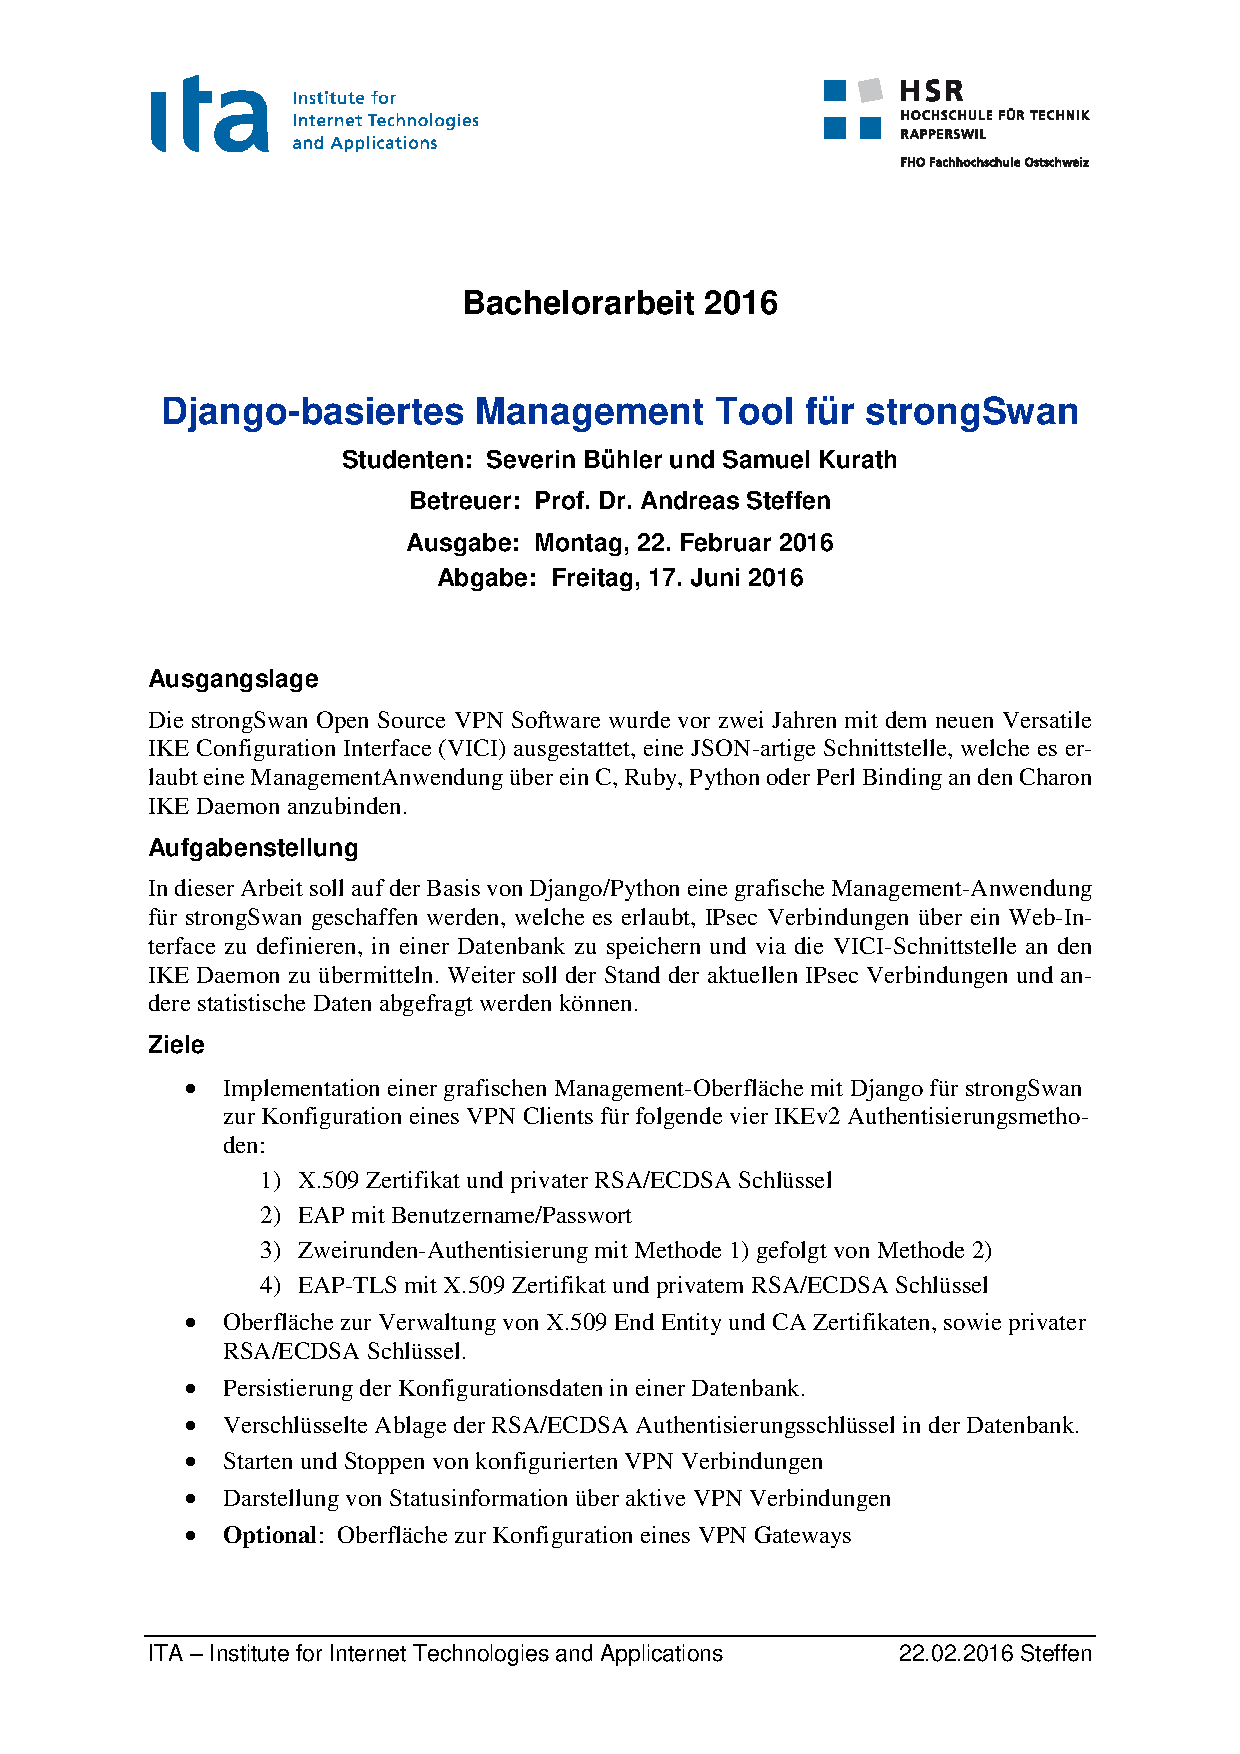
\includepdf[pages=-,offset=75 -75,frame,scale=.75,pagecommand={\section{Aufgabenstellung}}]{pdfs/Bachelorarbeit_2016_strongMan_Seite_1.pdf}
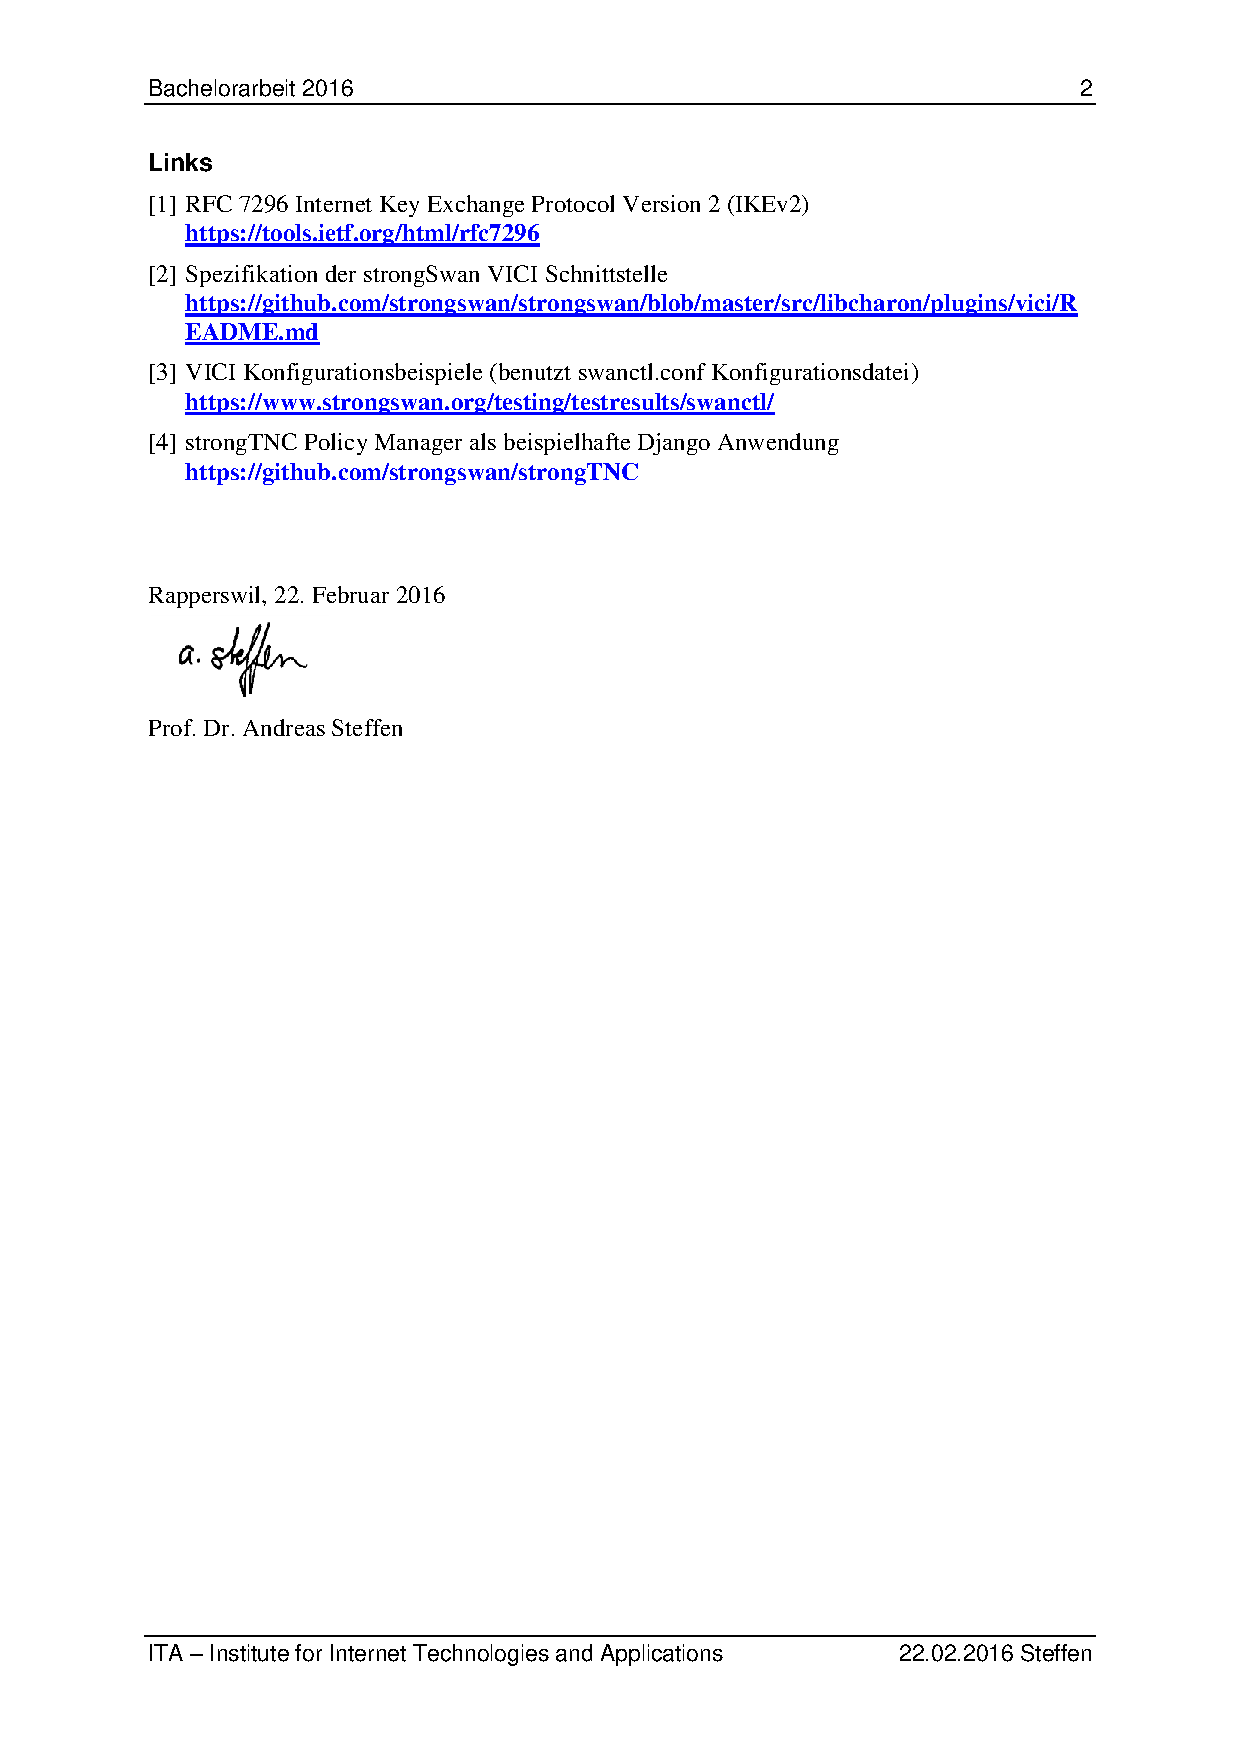
\includepdf[pages=-,offset=75 -75,frame,scale=.75,pagecommand={}]{pdfs/Bachelorarbeit_2016_strongMan_Seite_2.pdf}

% The main content
%%%%%%%%%%%%%%%%%%
\chapter{Analyse}
\newpage
\section{Einführung}
\subsection{Vision}
\label{subsec:vision}
\paragraph{Aktuell}
StrongSwan wird standardmässig per Konfigurationsdateien verwaltet, dies zielt stark auf eher versierte Nutzer und Administratoren ab.\\

\paragraph{Vision} 
Es soll eine Applikation entstehen, mit der dieser komplexe Prozess erleichtert wird. Dabei wir auf ein graphisches Interface gesetzt.\\
\section{Anforderungsspezifikation}
\subsection{Allgemeine Beschreibung}
Im generellen sind zwei Anwendungsszenarien denkbar:
\begin{itemize}
	\item VPN-Client
	\item VPN-Gateway
\end{itemize}
\medskip
Dabei ist der VPN-Client eine \textbf{Muss}-Anforderung und der VPN-Gateway eine \textbf{Kann}-Anforderung.
\medskip
\subsubsection{VPN-Client}
Die Applikation wird von einem Standard-Nutzer verwendet. Dieser soll VPN Tunnels zu Gateways konfigurieren können und die Tunnels starten und stoppen. Die Konfigurationsmöglichkeiten sind beschränkt, als Richtwert wird der strongSwan Android Client verwendet.\\


\subsubsection{VPN-Gateway}
Der Gateway ist auf Systemadministratoren ausgerichtet. Es soll möglich sein per grafischem Interface strongSwan zu konfigurieren und Tunnels einzurichten, welche als Gateway genutzt werden. 

\subsection{Use Case}
\subsubsection{Aktoren und Stakeholder}
\begin{table}[H]
\centering
    \begin{tabular}{|p{3cm}|p{9cm}|}
    \hline
    \rowcolor{lightblue}
    Aktor & Tätigkeit   \\ \hline
	User  & 
			\begin{itemize}
			\item Konfiguriert VPN-Tunnel als Client
    		\item Startet und stoppt VPN-Tunnel
		\end{itemize}	
	\\ \hline
	Administrator & 
			\begin{itemize}
			\item Konfiguriert VPN-Tunnel als Gateway
    		\item Startet und stoppt VPN-Tunnel
		\end{itemize}	
	\\ \hline
	\end{tabular}
    \caption[Aktoren und Stakeholder]{Aktoren und Stakeholder}
\end{table}




\subsubsection{Use Case Diagramm}
\begin{figure}[H]
\centering
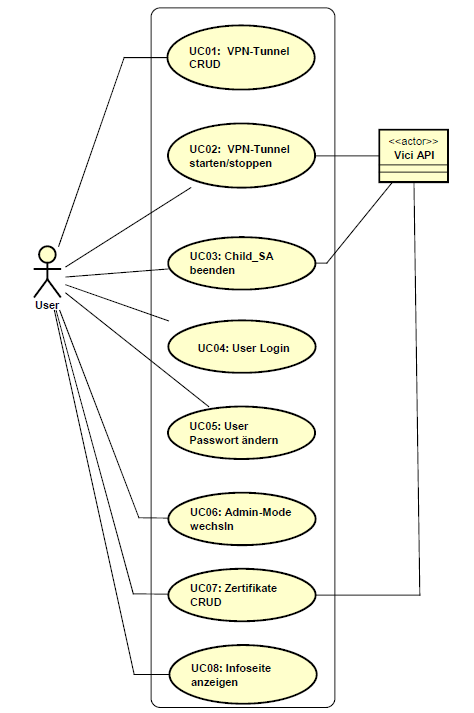
\includegraphics[width=350pt]{images/strongMan_usecase.png}
\caption[Use Case Diagramm]{Use Case Diagramm}
\end{figure}


\subsubsection{Use Cases Brief}
Alle hier definierten Use Cases haben auch ein entsprechendes Mockup im Anhang.
\paragraph{UC01: VPN-Tunnel CRUD}\mbox{} \\
Der User kann einen VPN-Tunnel erfassen / konfigurieren. Dabei hat er eine Auswahl von verschiedenen vordefinierten Tunneltypen. Jeder Tunneltyp hat eigene Konfigurationsfelder, die der User ausfüllen muss. Die Tunnel-Übersichtsseite stellt die Hauptseite der Applikation dar. Dort können die Tunnels bearbeitet und gelöscht werden.

\paragraph{UC02: VPN-Tunnel starten/stoppen}\mbox{} \\
Der User kann einen erfassten VPN-Tunnel starten und stoppen. Dabei wird die Konfiguration über die Vici API geladen. Falls ein VPN-Tunnel nicht aufgebaut werden kann, soll eine passende Fehlermeldung angezeigt werden. 

\paragraph{UC03: Child\_SA beenden}\mbox{} \\
Jeder VPN-Tunnel kann mehrere Child\_SA enthalten. Dieser werden in der Hauptseite angezeigt und können vom User beendet werden. Dieser Use Case interagiert mit der VICI Schnittstelle.

\paragraph{UC04: User Login}\mbox{} \\
Der User loggt sich zu Beginn beim Webseiten Aufruf mit einem Passwort ein. Es existiert dabei nur ein User mit Passwort.

\paragraph{UC05: User Passwort ändern}\mbox{} \\
Sobald der User eingeloggt ist, hat er die Möglichkeit, sein Passwort zu ändern. Dabei gibt er sein altes Passwort einmal und sein neues Passwort zweimal ein.

\paragraph{UC06: Admin-Mode wechseln}\mbox{} \\
Das Userinterface unterscheidet zwischen zwei Modis: User- \& Admin-Mode. Der Mode kann durch einem Klick auf einen Button gewechselt werden. Der Admin-Mode stellt einige Gateway-spezifische Funktionalitäten zusätzlich zur Verfügung, welche der User zur einfacheren Bedienung nicht sieht.

\paragraph{UC07: Zertifikate CRUD}\mbox{} \\
Dem User wird eine Zertifikatsverwaltung zur Verfügung gestellt. Er kann Zertifikate und Private Key's in den gängigen Formaten uploaden, anschauen, updaten (Passwort ändern) und wieder löschen. Die Dateien können mit einem Passwort verschlüsselt sein. Dieser Use Case interagiert unter Umständen mit der VICI Schnittstelle.

\paragraph{UC08: Infoseite anzeigen}\mbox{} \\
Die Infoseite zeigt dem eingeloggten User verschieden Informationen über das installierte System wie Charon Version, installierte Plugins usw.

\newpage





\input{chapter/Analyse/sequenzdiagramme}
\subsection{Architektur}

\subsubsection{Übersicht}
Die strongMan Applikation ist webbasiert, der Aufbau gliedert sich in folgende Komponenten.

\paragraph{Webbrowser} ist der Einstiegspunkt für den Benutzer und übernimmt die Darstellung mit Hilfe von HTML und CSS. Die Kommunikation findet per HTTP statt. Durch den Einsatz von Javascript ist auch ein wenig Logik eingebaut.  

\paragraph{Django Server} beinhaltet die eigentliche Business Logik,  stellt dem Webbrowser den Inhalt zur Verfügung, regelt die Kommunikation mit dem strongSwan per Unix Socket und nutzt zur Persisterung der Daten die Datenbank.

\paragraph{Database} beinhaltet die Konfigurationsangaben, sowie die Zertifikate.

\paragraph{strongSwan} baut die Ipsec-Tunnels auf und ab. Der Django Server nutzt die Vici-Schnittstelle um Konfiguration zu übergeben und die Verbindungen zu starten beziehungsweise zu stoppen. \\\\


\begin{figure}[H]
\centering
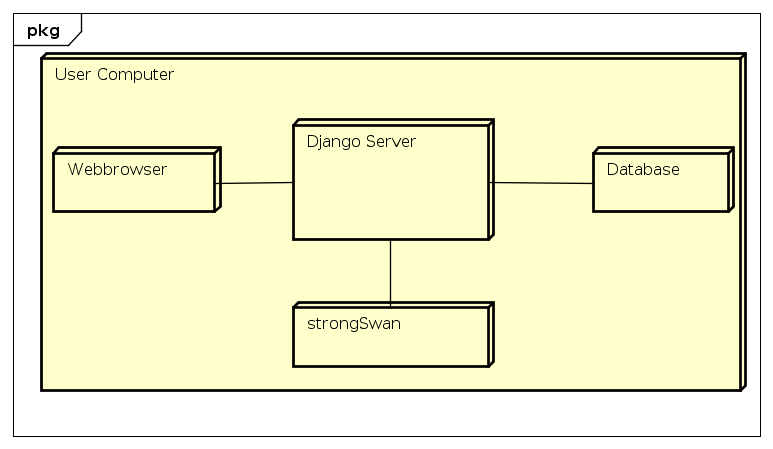
\includegraphics[width=360pt]{images/deployment.png}
\caption[Deployment]{Deployment}
\end{figure}

\subsection{Domain Model}

\begin{figure}[H]
\centering
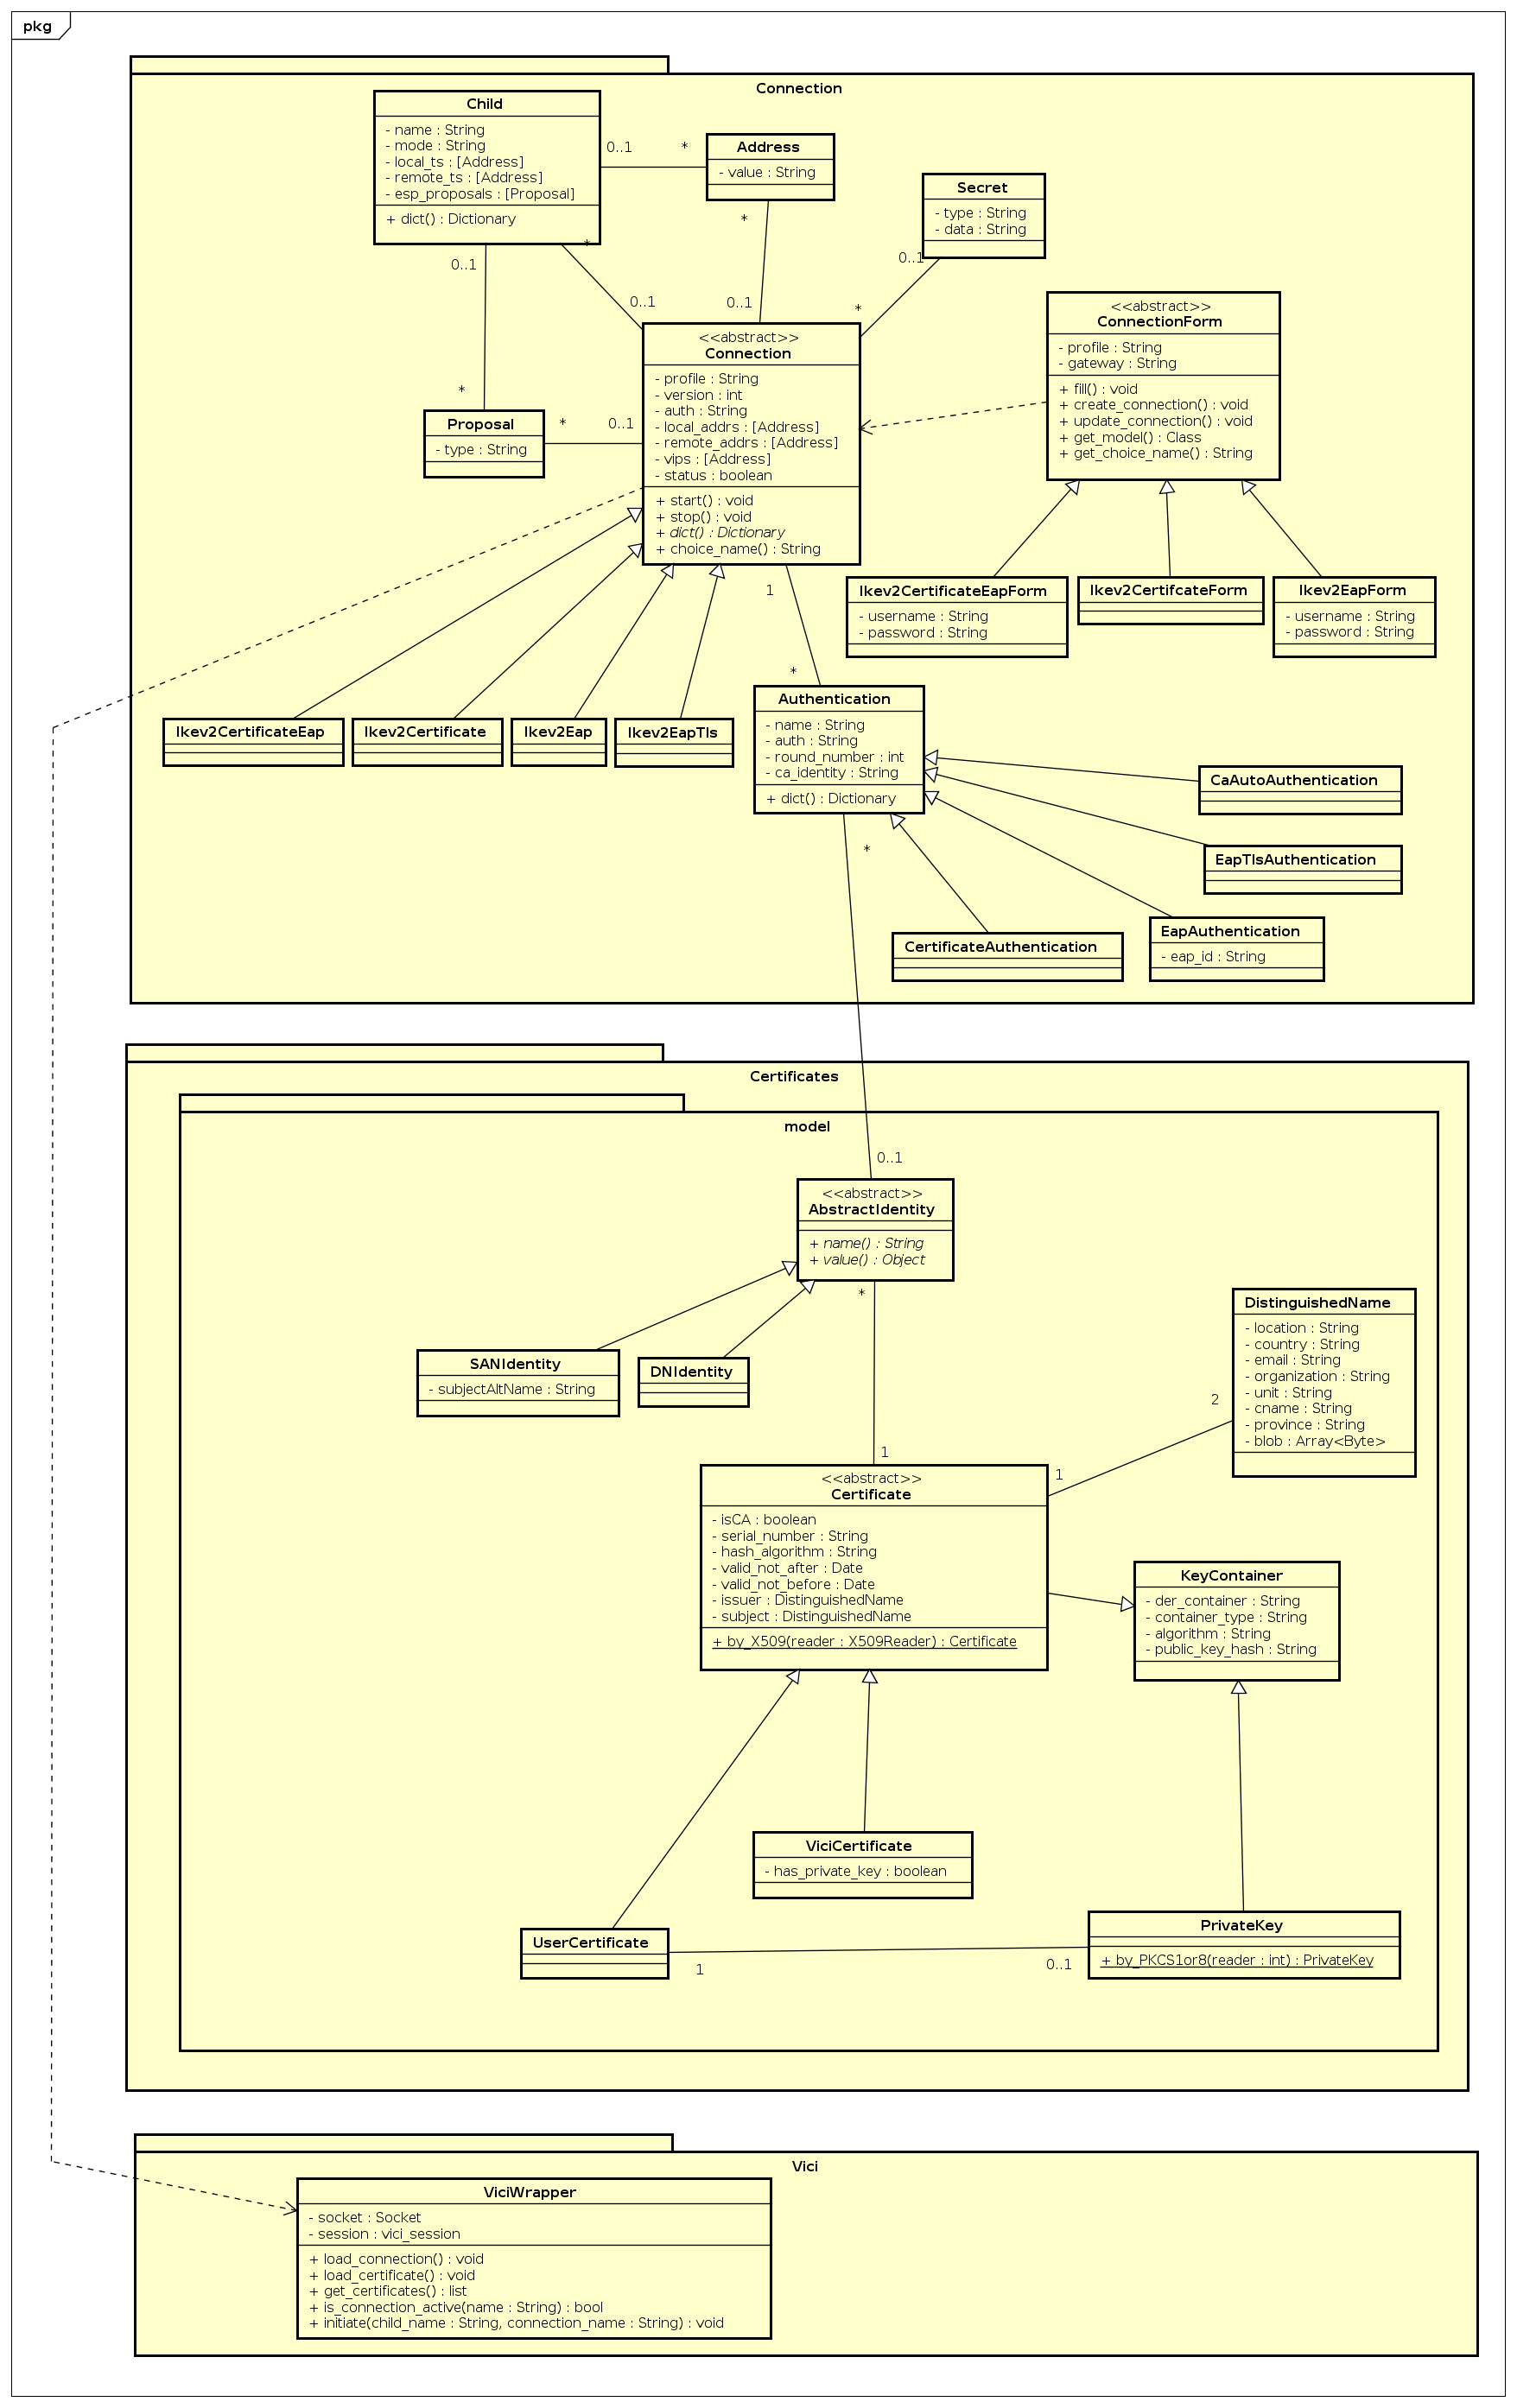
\includegraphics[width=420pt]{images/domain_model_strongman.png}
\caption[Domain Model]{Domain Model}
\end{figure}

Das Domain Model soll im Allgemeinen eine Abstraktion der Vici-Schnittstelle darstellen.
Dabei ist die Connection Klasse zentral. Damit die verschiedenen Authentisierungsmethoden unterstütz werden können, wird von Connection geerbt.

Weiter sind die Certificates ein essentieller Bestandteil, diese sind über die Hilfsklasse AbstractIdentity mit der Authentication verbunden, welche wiederum ein Verbindung zur Connection hat.

\newpage
\subsection{Nichtfunktionale Anforderungen}
\subsubsection{Funktionalität}
\paragraph{Sicherheit}
Änderung an den Daten der Anwendung dürfen nur authentifizierte Benutzer machen. Nicht authentifizierte Benutzer werden auf die Anmeldeseite weitergeleitet.

\paragraph{Sensitive Daten}
Kritische Daten sind das Passwort für den Benutzer/Adminstrator, die Private Keys und Secret Konfigurationsdaten (z.B. EAP Passwort). Die Private Key werden entschlüsselt und im Anschluss mit dem Password des Benutzers verschlüsselt in der Datenbank gespeichert.

\paragraph{Passwort Anforderungen}
\begin{itemize}
	\item minimal 8 Zeichen
	\item maximal 60 Zeichen
	\item minimal 1 Sonderzeichen und 1 Zahl
	\item minimal 1 Grossbuchstaben
	\item minimal 1 Kleinbuchstaben
\end{itemize}

\paragraph{Weitere Schutzmassnahmen}
\begin{itemize}
	\item Die Applikation muss vor SQL Injection sicher sein
	\item Um vor Cross Site Attacken sicher zu sein, werden CSFR Tokens verwendet
\end{itemize}

\paragraph{Interoperabilität}
Als externe Schnittstelle ist das Vici Interface aufzuzählen, dabei wir über Unix Sockets kommuniziert. StrongSwan bietet dazu schon eine Python Implementation an.
\paragraph{Richtigkeit}
Alle Eingabefehler werden validiert und auf deren Korrektheit überprüft.

\subsubsection{Zuverlässigkeit}

\paragraph{Wiederherstellbarkeit}
Nach einem Systemabsturz oder Stopp, soll die Anwendung ohne Komplikationen wieder gestartet werden können. Der User muss sich neu einloggen. Die Tunnels im Usermode werden beim Start der Applikation nicht direkt gestartet. Die Tunnels im Adminmode werden direkt gestartet.

\paragraph{Fehlertoleranz}
Bei einem Anwendungsfehler sollte nur die Operation des verursachten Benutzers abgebrochen werden. Andere Benutzer sollten vom Fehler nicht betroffen sein.\\
Bsp.: Bei fehlerhaften Löschen eines Zertifikates, sollen die Connections nicht gelöscht werden.
\subsubsection{Benutzbarkeit}

\paragraph{Erlernbarkeit}
Neue Benutzer sollten die grundlegenden Funktionen durch Verwenden der Anwendung und eines Tutorials erlernen können.

\paragraph{Bedienbarkeit}
Die Anwendung sollte leicht bedienbar sein. Die Applikation sollte sowohl auf einem Smartphone, wie auch auf einem Desktopcomputer bedienbar sein, weshalb wir mit einem responsiven Webdesign arbeiten. \\\\
Minimale Auflösung: 	640 × 960 px \\
Maximale Auflösung: 	1920 x 1080 px \\\\
Wir verwenden dabei 2 Skalierungsstufen (Smartphones, Desktopcomputer).

\paragraph{Robustheit}
Jedes Eingabefeld soll durch die Webseite validiert werden. Falsche Eingaben werden angezeigt, damit der Benutzer seine Eingabe korrigieren kann. Für jede falsche Eingabe soll eine kleiner Hilfetext erscheinen.

\paragraph{Effizienz}
Die Anwendung wird für einen zur gleichen Zeit arbeitenden User spezifiziert. Es können theoretisch mehrere User auf der Anwendung arbeiten, es existiert aber nur ein Userlogin und es können im schlimmsten Fall Race Conditions auftreten.
Die Ladezeit für die Anwendung soll für jede Operation unter 1 Sekunde bleiben. Bezüglich Geschwindigkeit muss das Projekt nicht spezifisch auf “langsame Devices” wie Router oder Raspberry Pi's achten.

\subsubsection{Änderbarkeit}
Die Applikation soll auch nach Projektabschluss betreubar sein. Daher sollen folgende Anforderungen erfüllt werden: 
\begin{itemize}
	\item Der Coding-Standard PEP8 für Python soll eingehalten werden.
	\item Klassen und nicht-triviale Methoden sollen im Code dokumentiert werden (Doc-Strings)
\end{itemize}

\paragraph{Modifizierbarkeit}
Es soll bei der Entwicklung darauf geachtet werden, zukünftige Erweiterungen nicht durch Design-Entscheide auszuschliessen.


\subsubsection{Übertragbarkeit}
Server: Die Anwendung muss mithilfe eines Django kompatiblen Webservers zum laufen gebracht werden. Zusätzlich zu den Django Anforderungen muss strongSwan mit der Vici Schnittstelle installiert sein.

Client: Auf dem Client muss ein aktueller Browser mit HTML5 und Javascript Unterstützung installiert sein. Die Applikation wird mit Google Chrome 49 und Firefox 45 getestet.


\paragraph{Internationalization}
Die Applikation ist in der Englischen Sprache verfügbar.

\paragraph{Testing}
Die Hauptfunktionen im Projekt sollten mittels Unit Tests getestet werden. Die Haupt Use Cases müssen mit Integration Tests überprüft werden. Es sind keine Stresstests mit Loadtesting Frameworks wie Gatling vorgesehen.




\section{Umsetzungskonzept}
\label{sec:umsetzung}
Die Grundidee für die Umsetzung des Management Tools:
\begin{enumerate}
	\item 1
	\item 2
\end{enumerate}


\section{Mockups}
Um allen Projektbeteiligten ein Bild der zukünftigen Applikation zu vermitteln, sind für die wichtigsten Seiten Mockups entstanden. In diesem Abschnitt wird auf zwei Ansichten in der Connection Verwaltung eingegangen. Alle anderen Mockups sind im Anhang auf der Seite \pageref{Mockups} ersichtlich.

\subsection{Connection Übersicht}
\begin{figure}[H]
	\centering
	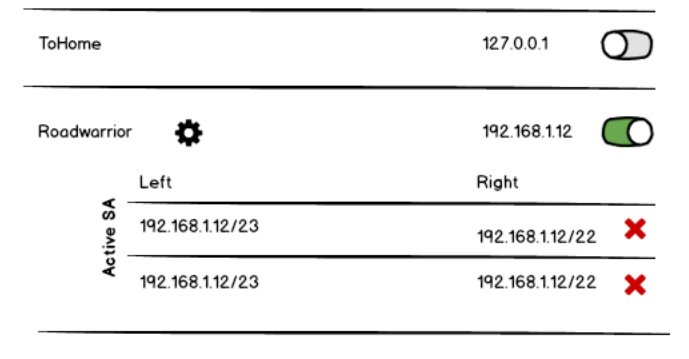
\includegraphics[width=330pt]{images/mockups/short_con_overview.jpg}
	\caption{Ausschnitt aus der Connection Übersicht}
\end{figure}

Die erstellten Verbindungen werden in Zeilenform untereinander angeordnet. Es gibt einen zentralen Toggle Button, der die Verbindung aktiviert/deaktiviert und gleichzeitig den Verbindungsstatus anzeigt. Sobald die Verbindung gestartet wurde, wird die Verbindungszeile erweitert und die aktiven SA's angezeigt.

\subsection{Connection hinzufügen}
\noindent\begin{minipage}{0.55\textwidth}
    \begin{figure}[H]
    	\centering
    	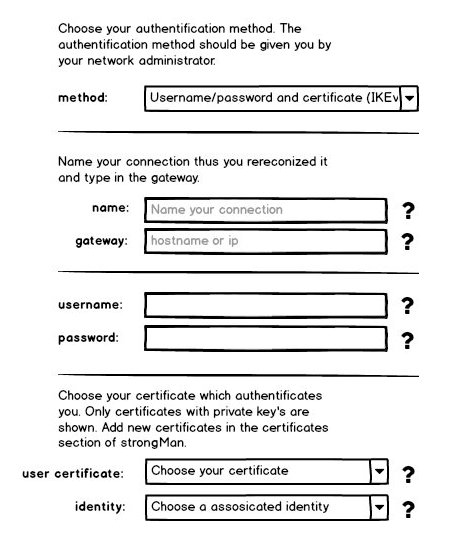
\includegraphics[width=240pt]{images/mockups/short_con_config.jpg}
    	\caption{Ausschnitt aus dem Connection hinzufügen}
    \end{figure}
\end{minipage}
\hfill
\begin{minipage}{0.45\textwidth}
Nachdem der Benutzer die Authentifizierungsmethod ausgewählt hat (hier nicht ersichtlich), erscheinen unterhalb die entsprechenden Eingabefelder.

Das Konfigurieren einer Verbindung wurde so einfach wie möglich gestaltet. Der Benutzer soll kurz vor jeder Eingabe informiert werden, welche Nutzen das entsprechende Feld hat und sich bei Schwierigkeiten an Hilfetexten informieren können (Klick auf die Fragezeichen).
\end{minipage}


\section{Usability Tests}
\section{Evaluation Usermanagement}
Da mit Hilfe von stongSwan VPN Tunnels zu schützenswerten Daten ermöglicht werden, sollt auch die Applikation strongMan mit einer Authentifizierung versehen werden.
\subsection{Anforderungen}
\begin{itemize}
	\item Benutzer hat ohne sich einzuloggen keinen Zugriff auf die Applikation
	\item Benutzer hat die Möglichkeit sein Passwort zu ändern
\end{itemize}

\subsection{Varianten}
\begin{itemize}
	\item Ein vorkonfigurierter Benutzer
	\item Mehrere Benutzer
	\item Benutzer des Systems verwenden
\end{itemize}
\subsection{Auswertung}
\begin{table}[H]
\centering
    \begin{tabular}{|l|l|l|l|}
    \hline
    \rowcolor{lightblue}
    Variante & Implementierung & Framework Unterstützung & Komplexität   \\ \hline
	Ein vorkonfigurierter Benutzer	&	leicht	& gegeben	&	niedrig	\\ \hline
		Mehrere Benutzer	&	mittel	& gegeben	&	mittel	\\ \hline
		Benutzer des Systems verwenden	&	schwer	& nicht gegeben	&	hoch	\\ \hline	
	\end{tabular}
    \caption[Evaluation Usermanagement]{Evaluation Usermanagement}
\end{table}

\decision{Evaluation Usermanagement}
Durch das Vergleichen der verschieden Varianten und in Absprache mit den Betreuern hat sich 'Ein vorkonfigurierter Benutzer' als klarer Favorit herausgestellt. Dabei wir ein Standard Benutzer während er Installation der Applikation erstellt und dessen Passwort kann im Anschluss geändert werden.

\section{Evaluation Zertifikatsbibliothek}
Um VPN-Verbindungen mit Zertifikaten abzusichern, muss das strongSwan Management Interface mit Zertifikaten umgehen können. Dabei müssen verschiedene Formate unterstützt, ausgelesen und entsprechend Ihrem Inhalt an die Vici-Schnittstelle geliefert werden.
\subsection{Übersicht}
\subsubsection{ASN.1 Schemas}
In der Welt der asymmetrischen Verschlüsslung werden alle nötigen Daten mithilfe einer ASN.1 Struktur abgelegt. Der ASN.1 Standard stellt Datentypen und Datenstrukturen zur Verfügung, um Informationen mithilfe eines Schemas abzulegen. Über die Zeit sind verschiedene RFC’s entstanden, die ASN.1 Schemas definieren. Unten aufgelistet sind die Standards, welche wir in unserem Projekt berücksichtigen. \medskip

\begin{table}[H]
\centering
    \begin{tabular}{|l|p{12cm}|l|}
    \hline
    \rowcolor{lightblue}
    Standard & Inhalt & Forderung   \\ \hline
	PKCS\#1	&	Private Schlüssel der verschiedene Algorithmen RSA, DSA, ECDSA. Können mit einem Passwort verschlüsselt sein.	& Muss \\ \hline	
		PKCS\#8	&	Gleich wie PKCS\#1, nur hier in einer besser verständlichen Form.	& Muss \\ \hline	
		X.509	&	Zertifikatsstandard mit allen Informationen zum Eigner. Unverschlüsselt.	& Muss \\ \hline
		PKCS\#12	&	Container mit Zertifikaten und Private Keys. Kann verschlüsselt sein.	& Kann \\ \hline		
	\end{tabular}
    \caption[ASN.1 Schemas]{ASN.1 Schemas}
\end{table}

\subsubsection{Encoding}
Die ASN.1 Strukturen werden nicht direkt in die Dateien abgespeichert, sondern zuerst in einem speziellen Format codiert. Dabei sind zwei verschiedene Standards üblich. \medskip

\begin{table}[H]
\centering
    \begin{tabular}{|l|p{12cm}|l|}
    \hline
    \rowcolor{lightblue}
    Standard & Inhalt & Forderung   \\ \hline
	DER	&	Binär kodiert und somit nicht in einem Editor lesbar. Dateiendung .der.	& Muss \\ \hline	
		PEM	&	
Base64 encodet in ASCII Zeichen. Dateiendung .pem. Openssl nutzt PEM als Standardencoding.	& Muss \\ \hline		
	\end{tabular}
    \caption[Encoding]{Encoding}
\end{table}

\subsubsection{Verschlüsslung}
Die Dateien mit Private Keys (PKCS\#1, PKCS\#8 und PKCS\#12) können verschlüsselt sein. Dabei kommen verschiedene symmetrische Verschlüsslungen zum Einsatz, die mit einem Userpasswort entschlüsselt werden.


\subsubsection{Anforderungen}
In dieser Evaluation soll eine Python Crypto Bibliothek gefunden werden, mit der man grundlegende Informationen wie CNAME und ASN.1 Schema auslesen kann. Mithilfe der Anforderungstabelle unten soll eine passende Bibliothek gefunden werden.

\paragraph{Muss Anforderungen}
\begin{itemize}
	\item Unterscheidung Private Key / Zertifikat
	\item Erkennung von CA Zertifikaten
	\item Unterstützt alle obigen ASN.1 Schemas
	\item Unterstützt PEM und DER Encoding
	\item Aus X.509 können Infos wie der CNAME ausgelesen werden	
\end{itemize}

\paragraph{Kann Anforderungen}
\begin{itemize}
	\item Private Keys können entschlüsselt werden	
	\item Bibliothek ist pure Python (Keine Kompilation bei Installation)
	\item PKCS\#12 wird unterstützt
	\item Matching zwischen Public und Private Key ist möglich
	\item Einfaches API
\end{itemize}

\subsubsection{Kandidaten}
\subsubsection{Pyasn1}
\begin{table}[H]
\centering
    \begin{tabular}{|p{12cm}|l|l|}
    \hline
    \rowcolor{lightblue}
    Anforderungen & Muss / Kann & Erfüllt   \\ \hline
	Unterscheidung Private Key / Zertifikat	&	Muss & x \\ \hline	
	Erkennung von CA Zertifikaten	&	Muss	& x \\ \hline	
	Unterstützt alle obigen ASN.1 Schemas	&	Muss	& x \\ \hline		
	Unterstützt PEM und DER Encoding	&	Muss	& x \\ \hline	
	Aus X.509 können Infos wie der CNAME ausgelesen werden &	Muss	& x \\ \hline	
	Private Keys können entschlüsselt werden &	Kann &  \\ \hline
	Bibliothek ist pure Python (Keine Kompilation bei Installation) &	Kann	&  x \\ \hline
	PKCS\#12 wird unterstützt &	Kann &  \\ \hline
	Matching zwischen Public und Private Key ist möglich &	Kann &  \\ \hline
	Einfaches API &	Kann &  \\ \hline
	\end{tabular}
    \caption[Pyasn1]{Pyasn1}
\end{table}

Pyasn1 stellt einzelnen ASN.1 Schemas für die dekodierung von ASN.1 Dateien zur Verfügung. Einzelne Standards wie X.509 sind schon implementiert, jedoch ist man selbst verantwortlich, das richtige Schema zu der entsprechenden Datei zu finden. Das API ist sehr kompliziert und der Programmieraufwand für die Unterstützung alles nötigen Formate ist gross.


\subsubsection{Cryptography}
\begin{table}[H]
\centering
    \begin{tabular}{|p{12cm}|l|l|}
    \hline
    \rowcolor{lightblue}
    Anforderungen & Muss / Kann & Erfüllt   \\ \hline
	Unterscheidung Private Key / Zertifikat	&	Muss &  \\ \hline	
	Erkennung von CA Zertifikaten	&	Muss	& x \\ \hline	
	Unterstützt alle obigen ASN.1 Schemas	&	Muss	&  \\ \hline		
	Unterstützt PEM und DER Encoding	&	Muss	&  x\\ \hline	
	Aus X.509 können Infos wie der CNAME ausgelesen werden &	Muss	& x \\ \hline	
	Private Keys können entschlüsselt werden &	Kann &  \\ \hline
	Bibliothek ist pure Python (Keine Kompilation bei Installation) &	Kann	&   \\ \hline
	PKCS\#12 wird unterstützt &	Kann &  \\ \hline
	Matching zwischen Public und Private Key ist möglich &	Kann &  \\ \hline
	Einfaches API &	Kann & x \\ \hline
	\end{tabular}
    \caption[Cryptography]{Cryptography}
\end{table}

Cryptography ist ein Python Bibliothek mit dem Fokus auf komfortabler Cryptography in Python. Es hat eine tolle Unterstützung für X.509 Zertifikate. Man kann Private Keys generieren, ein CSR erstellen und sogar CSR signieren. Im Hintergrund verwendet es OpenSSL. Nichts desto trotz bietet es keinen Support ausserhalb vom X.509 und ist somit unbrauchbar für unsere Zwecke.


\subsubsection{Pycrypto}
\begin{table}[H]
\centering
    \begin{tabular}{|p{12cm}|l|l|}
    \hline
    \rowcolor{lightblue}
    Anforderungen & Muss / Kann & Erfüllt   \\ \hline
	Unterscheidung Private Key / Zertifikat	&	Muss & x \\ \hline	
	Erkennung von CA Zertifikaten	&	Muss	& x \\ \hline	
	Unterstützt alle obigen ASN.1 Schemas	&	Muss	& x \\ \hline		
	Unterstützt PEM und DER Encoding	&	Muss	&  x \\ \hline	
	Aus X.509 können Infos wie der CNAME ausgelesen werden &	Muss	& x \\ \hline	
	Private Keys können entschlüsselt werden &	Kann &  \\ \hline
	Bibliothek ist pure Python (Keine Kompilation bei Installation) &	Kann	&   \\ \hline
	PKCS\#12 wird unterstützt &	Kann &  \\ \hline
	Matching zwischen Public und Private Key ist möglich &	Kann &  x \\ \hline
	Einfaches API &	Kann &  \\ \hline
	\end{tabular}
    \caption[Pycrypto]{Pycrypto}
\end{table}

Pycrypto unterstützt alle geforderten Formate inkl. Verschlüsslung. Es basiert auf der OpenSSL Bibliothek, welche davor zuerst installiert werden muss. Die Anwendung von Pycrypto erfordert jedoch einiges an Code, um jedes Format durchzutesten und um die entsprechenden Formate zu erkennen.


\subsubsection{Oscrypto}
\begin{table}[H]
\centering
    \begin{tabular}{|p{12cm}|l|l|}
    \hline
    \rowcolor{lightblue}
    Anforderungen & Muss / Kann & Erfüllt   \\ \hline
	Unterscheidung Private Key / Zertifikat	&	Muss & x \\ \hline	
	Erkennung von CA Zertifikaten	&	Muss	& x \\ \hline	
	Unterstützt alle obigen ASN.1 Schemas	&	Muss	& x \\ \hline		
	Unterstützt PEM und DER Encoding	&	Muss	&  x \\ \hline	
	Aus X.509 können Infos wie der CNAME ausgelesen werden &	Muss	& x \\ \hline	
	Private Keys können entschlüsselt werden &	Kann &  x \\ \hline
	Bibliothek ist pure Python (Keine Kompilation bei Installation) &	Kann	&  ~ \\ \hline
	PKCS\#12 wird unterstützt &	Kann & x \\ \hline
	Matching zwischen Public und Private Key ist möglich &	Kann & ~  \\ \hline
	Einfaches API &	Kann & x \\ \hline
	\end{tabular}
    \caption[Pycrypto]{Pycrypto}
\end{table}

Oscrypto ist eine neu entstandene Crypto Bibliothek für Python. Es unterstützt alle nötigen Formate inkl. Verschlüsslung. Die meisten Funktionen können ohne die OpenSSL Bibliothek im Hintergrund verwendet werden. Mit wenigen Befehlen kann oscrypto alle nötigen Formate lesen. Es müssen nicht alle durch probiert werden.\\
\medskip

\decision{Evaluation Zertifikatsbibliothek}
Der Entscheid fiehl klar auf oscrypto. Oscrypto ist eine pure Python Bibliothek, welche verschiedene Cryptofunktionen anbietet. Für das Parsen und Lesen von Keycontainer wrappt oscrypto die asn1crypto Bibliothek (auch pure Python). Für andere Cryptofunktionen wrappt oscrypto die standartmässig installierte OpenSSL Library, welche wir aber in dieser Arbeit nicht brauchen.
Mithilfe dieser Library ist nun ein komfortables Arbeiten mit allen oben aufgeführen Keycontainern möglich, ohne je einen nicht-Python Kompiler anwerfen zu müssen. 

\newpage	
\chapter{Technischer Bericht}
\newpage 
\section{Evaluation Usermanagement}
Da mit Hilfe von stongSwan VPN Tunnels zu schützenswerten Daten ermöglicht werden, sollt auch die Applikation strongMan mit einer Authentifizierung versehen werden.
\subsection{Anforderungen}
\begin{itemize}
	\item Benutzer hat ohne sich einzuloggen keinen Zugriff auf die Applikation
	\item Benutzer hat die Möglichkeit sein Passwort zu ändern
\end{itemize}

\subsection{Varianten}
\begin{itemize}
	\item Ein vorkonfigurierter Benutzer
	\item Mehrere Benutzer
	\item Benutzer des Systems verwenden
\end{itemize}
\subsection{Auswertung}
\begin{table}[H]
\centering
    \begin{tabular}{|l|l|l|l|}
    \hline
    \rowcolor{lightblue}
    Variante & Implementierung & Framework Unterstützung & Komplexität   \\ \hline
	Ein vorkonfigurierter Benutzer	&	leicht	& gegeben	&	niedrig	\\ \hline
		Mehrere Benutzer	&	mittel	& gegeben	&	mittel	\\ \hline
		Benutzer des Systems verwenden	&	schwer	& nicht gegeben	&	hoch	\\ \hline	
	\end{tabular}
    \caption[Evaluation Usermanagement]{Evaluation Usermanagement}
\end{table}

\decision{Evaluation Usermanagement}
Durch das Vergleichen der verschieden Varianten und in Absprache mit den Betreuern hat sich 'Ein vorkonfigurierter Benutzer' als klarer Favorit herausgestellt. Dabei wir ein Standard Benutzer während er Installation der Applikation erstellt und dessen Passwort kann im Anschluss geändert werden.

\section{Evaluation Zertifikatsbibliothek}
Um VPN-Verbindungen mit Zertifikaten abzusichern, muss das strongSwan Management Interface mit Zertifikaten umgehen können. Dabei müssen verschiedene Formate unterstützt, ausgelesen und entsprechend Ihrem Inhalt an die Vici-Schnittstelle geliefert werden.
\subsection{Übersicht}
\subsubsection{ASN.1 Schemas}
In der Welt der asymmetrischen Verschlüsslung werden alle nötigen Daten mithilfe einer ASN.1 Struktur abgelegt. Der ASN.1 Standard stellt Datentypen und Datenstrukturen zur Verfügung, um Informationen mithilfe eines Schemas abzulegen. Über die Zeit sind verschiedene RFC’s entstanden, die ASN.1 Schemas definieren. Unten aufgelistet sind die Standards, welche wir in unserem Projekt berücksichtigen. \medskip

\begin{table}[H]
\centering
    \begin{tabular}{|l|p{12cm}|l|}
    \hline
    \rowcolor{lightblue}
    Standard & Inhalt & Forderung   \\ \hline
	PKCS\#1	&	Private Schlüssel der verschiedene Algorithmen RSA, DSA, ECDSA. Können mit einem Passwort verschlüsselt sein.	& Muss \\ \hline	
		PKCS\#8	&	Gleich wie PKCS\#1, nur hier in einer besser verständlichen Form.	& Muss \\ \hline	
		X.509	&	Zertifikatsstandard mit allen Informationen zum Eigner. Unverschlüsselt.	& Muss \\ \hline
		PKCS\#12	&	Container mit Zertifikaten und Private Keys. Kann verschlüsselt sein.	& Kann \\ \hline		
	\end{tabular}
    \caption[ASN.1 Schemas]{ASN.1 Schemas}
\end{table}

\subsubsection{Encoding}
Die ASN.1 Strukturen werden nicht direkt in die Dateien abgespeichert, sondern zuerst in einem speziellen Format codiert. Dabei sind zwei verschiedene Standards üblich. \medskip

\begin{table}[H]
\centering
    \begin{tabular}{|l|p{12cm}|l|}
    \hline
    \rowcolor{lightblue}
    Standard & Inhalt & Forderung   \\ \hline
	DER	&	Binär kodiert und somit nicht in einem Editor lesbar. Dateiendung .der.	& Muss \\ \hline	
		PEM	&	
Base64 encodet in ASCII Zeichen. Dateiendung .pem. Openssl nutzt PEM als Standardencoding.	& Muss \\ \hline		
	\end{tabular}
    \caption[Encoding]{Encoding}
\end{table}

\subsubsection{Verschlüsslung}
Die Dateien mit Private Keys (PKCS\#1, PKCS\#8 und PKCS\#12) können verschlüsselt sein. Dabei kommen verschiedene symmetrische Verschlüsslungen zum Einsatz, die mit einem Userpasswort entschlüsselt werden.


\subsubsection{Anforderungen}
In dieser Evaluation soll eine Python Crypto Bibliothek gefunden werden, mit der man grundlegende Informationen wie CNAME und ASN.1 Schema auslesen kann. Mithilfe der Anforderungstabelle unten soll eine passende Bibliothek gefunden werden.

\paragraph{Muss Anforderungen}
\begin{itemize}
	\item Unterscheidung Private Key / Zertifikat
	\item Erkennung von CA Zertifikaten
	\item Unterstützt alle obigen ASN.1 Schemas
	\item Unterstützt PEM und DER Encoding
	\item Aus X.509 können Infos wie der CNAME ausgelesen werden	
\end{itemize}

\paragraph{Kann Anforderungen}
\begin{itemize}
	\item Private Keys können entschlüsselt werden	
	\item Bibliothek ist pure Python (Keine Kompilation bei Installation)
	\item PKCS\#12 wird unterstützt
	\item Matching zwischen Public und Private Key ist möglich
	\item Einfaches API
\end{itemize}

\subsubsection{Kandidaten}
\subsubsection{Pyasn1}
\begin{table}[H]
\centering
    \begin{tabular}{|p{12cm}|l|l|}
    \hline
    \rowcolor{lightblue}
    Anforderungen & Muss / Kann & Erfüllt   \\ \hline
	Unterscheidung Private Key / Zertifikat	&	Muss & x \\ \hline	
	Erkennung von CA Zertifikaten	&	Muss	& x \\ \hline	
	Unterstützt alle obigen ASN.1 Schemas	&	Muss	& x \\ \hline		
	Unterstützt PEM und DER Encoding	&	Muss	& x \\ \hline	
	Aus X.509 können Infos wie der CNAME ausgelesen werden &	Muss	& x \\ \hline	
	Private Keys können entschlüsselt werden &	Kann &  \\ \hline
	Bibliothek ist pure Python (Keine Kompilation bei Installation) &	Kann	&  x \\ \hline
	PKCS\#12 wird unterstützt &	Kann &  \\ \hline
	Matching zwischen Public und Private Key ist möglich &	Kann &  \\ \hline
	Einfaches API &	Kann &  \\ \hline
	\end{tabular}
    \caption[Pyasn1]{Pyasn1}
\end{table}

Pyasn1 stellt einzelnen ASN.1 Schemas für die dekodierung von ASN.1 Dateien zur Verfügung. Einzelne Standards wie X.509 sind schon implementiert, jedoch ist man selbst verantwortlich, das richtige Schema zu der entsprechenden Datei zu finden. Das API ist sehr kompliziert und der Programmieraufwand für die Unterstützung alles nötigen Formate ist gross.


\subsubsection{Cryptography}
\begin{table}[H]
\centering
    \begin{tabular}{|p{12cm}|l|l|}
    \hline
    \rowcolor{lightblue}
    Anforderungen & Muss / Kann & Erfüllt   \\ \hline
	Unterscheidung Private Key / Zertifikat	&	Muss &  \\ \hline	
	Erkennung von CA Zertifikaten	&	Muss	& x \\ \hline	
	Unterstützt alle obigen ASN.1 Schemas	&	Muss	&  \\ \hline		
	Unterstützt PEM und DER Encoding	&	Muss	&  x\\ \hline	
	Aus X.509 können Infos wie der CNAME ausgelesen werden &	Muss	& x \\ \hline	
	Private Keys können entschlüsselt werden &	Kann &  \\ \hline
	Bibliothek ist pure Python (Keine Kompilation bei Installation) &	Kann	&   \\ \hline
	PKCS\#12 wird unterstützt &	Kann &  \\ \hline
	Matching zwischen Public und Private Key ist möglich &	Kann &  \\ \hline
	Einfaches API &	Kann & x \\ \hline
	\end{tabular}
    \caption[Cryptography]{Cryptography}
\end{table}

Cryptography ist ein Python Bibliothek mit dem Fokus auf komfortabler Cryptography in Python. Es hat eine tolle Unterstützung für X.509 Zertifikate. Man kann Private Keys generieren, ein CSR erstellen und sogar CSR signieren. Im Hintergrund verwendet es OpenSSL. Nichts desto trotz bietet es keinen Support ausserhalb vom X.509 und ist somit unbrauchbar für unsere Zwecke.


\subsubsection{Pycrypto}
\begin{table}[H]
\centering
    \begin{tabular}{|p{12cm}|l|l|}
    \hline
    \rowcolor{lightblue}
    Anforderungen & Muss / Kann & Erfüllt   \\ \hline
	Unterscheidung Private Key / Zertifikat	&	Muss & x \\ \hline	
	Erkennung von CA Zertifikaten	&	Muss	& x \\ \hline	
	Unterstützt alle obigen ASN.1 Schemas	&	Muss	& x \\ \hline		
	Unterstützt PEM und DER Encoding	&	Muss	&  x \\ \hline	
	Aus X.509 können Infos wie der CNAME ausgelesen werden &	Muss	& x \\ \hline	
	Private Keys können entschlüsselt werden &	Kann &  \\ \hline
	Bibliothek ist pure Python (Keine Kompilation bei Installation) &	Kann	&   \\ \hline
	PKCS\#12 wird unterstützt &	Kann &  \\ \hline
	Matching zwischen Public und Private Key ist möglich &	Kann &  x \\ \hline
	Einfaches API &	Kann &  \\ \hline
	\end{tabular}
    \caption[Pycrypto]{Pycrypto}
\end{table}

Pycrypto unterstützt alle geforderten Formate inkl. Verschlüsslung. Es basiert auf der OpenSSL Bibliothek, welche davor zuerst installiert werden muss. Die Anwendung von Pycrypto erfordert jedoch einiges an Code, um jedes Format durchzutesten und um die entsprechenden Formate zu erkennen.


\subsubsection{Oscrypto}
\begin{table}[H]
\centering
    \begin{tabular}{|p{12cm}|l|l|}
    \hline
    \rowcolor{lightblue}
    Anforderungen & Muss / Kann & Erfüllt   \\ \hline
	Unterscheidung Private Key / Zertifikat	&	Muss & x \\ \hline	
	Erkennung von CA Zertifikaten	&	Muss	& x \\ \hline	
	Unterstützt alle obigen ASN.1 Schemas	&	Muss	& x \\ \hline		
	Unterstützt PEM und DER Encoding	&	Muss	&  x \\ \hline	
	Aus X.509 können Infos wie der CNAME ausgelesen werden &	Muss	& x \\ \hline	
	Private Keys können entschlüsselt werden &	Kann &  x \\ \hline
	Bibliothek ist pure Python (Keine Kompilation bei Installation) &	Kann	&  ~ \\ \hline
	PKCS\#12 wird unterstützt &	Kann & x \\ \hline
	Matching zwischen Public und Private Key ist möglich &	Kann & ~  \\ \hline
	Einfaches API &	Kann & x \\ \hline
	\end{tabular}
    \caption[Pycrypto]{Pycrypto}
\end{table}

Oscrypto ist eine neu entstandene Crypto Bibliothek für Python. Es unterstützt alle nötigen Formate inkl. Verschlüsslung. Die meisten Funktionen können ohne die OpenSSL Bibliothek im Hintergrund verwendet werden. Mit wenigen Befehlen kann oscrypto alle nötigen Formate lesen. Es müssen nicht alle durch probiert werden.\\
\medskip

\decision{Evaluation Zertifikatsbibliothek}
Der Entscheid fiehl klar auf oscrypto. Oscrypto ist eine pure Python Bibliothek, welche verschiedene Cryptofunktionen anbietet. Für das Parsen und Lesen von Keycontainer wrappt oscrypto die asn1crypto Bibliothek (auch pure Python). Für andere Cryptofunktionen wrappt oscrypto die standartmässig installierte OpenSSL Library, welche wir aber in dieser Arbeit nicht brauchen.
Mithilfe dieser Library ist nun ein komfortables Arbeiten mit allen oben aufgeführen Keycontainern möglich, ohne je einen nicht-Python Kompiler anwerfen zu müssen. 
\section{Authentiserungsmethoden}
Die Konfigurationsmöglichkeiten der strongSwan Open Source VPN Software sind enorm. Damit das Erfassen der Verbindungsdaten nicht all zu unübersichtlich wird, beschränken wir uns auf die häufigst verwendeten Szenarien.

\begin{enumerate}
	\item X.509 Zertifikat und privater RSA/ECDSA Schlüssel
	\item EAP mit Benutzername/Passwort
	\item Zweirunden-Authentisierung mit Methode 1) gefolgt von Methode 2)
	\item EAP-TLS mit X.509 Zertifikat und privatem RSA/ECDSA Schlüssel
\end{enumerate}

Nachfolgend wird auf die jeweiligen Authentiserungsmethoden im Detail eingegangen. Bei der Verwendeten Notation der Konfiguration handelt es sich um Python ordered Dictionaries.\\
Die Clientseite wurde mit Hilfe der strongMan Applikation erstellt. Die Serverseite dient als Pendant dazu und ist als ein funktionstüchtiges Beispiel aufgeführt.

\subsubsection{Konfiguration}
Die Tabelle Konfiguration beschreibt einige Key Parameter, welche durch die strongMan Applikation gesetzt werden. Eine komplette Übersicht über die Paramter findet sich im strongSwan Repository auf Github\footnote{\url{https://github.com/strongswan/strongswan/tree/master/src/libcharon/plugins/vici}}, weiter kann die Dokumentation von swanctl\footnote{\url{https://wiki.strongswan.org/projects/strongswan/wiki/Swanctlconf}} als Hilfestellung hinzugezogen werden.\\
\begin{table}[H]
\centering
    \begin{tabular}{|p{0.2\textwidth}|p{0.2\textwidth}|p{0.5\textwidth}|}
    \hline
    \rowcolor{lightblue}
    Parameter & Wert & Erklärung \\ \hline
	vips	&	0.0.0.0,  :: & Virtuelle IP, welche dem Client vom Server zugewiesen wird. 0.0.0.0 und :: dienen als Wildcard-Adressen für IPv4 und IPv6, damit wird jede virtuelle IP akzeptiert.	\\ \hline
	version & 2 & IKE Version, es wird nur die Version 2 von strongMan verwendet \\ \hline
	auth & pubkey, eap, eap-tls & Definiert die verwendete Authentisierungsmethode. \\ \hline
	round & 1, 2 & Wird von Certificate + EAP benötigt, da es zwei Authentiserungsrunden hat. Der Parameter wird erst ab strongSwan Version 5.4.0 unterstützt. \\ \hline
	certs & Bytes & Byte Repräsentation des Benutzer-Zertifikates	\\ \hline
	cacerts & Bytes & Byte Repräsentation des Server-Zertifikates	\\ \hline
	\end{tabular}
    \caption[Konfiguration]{Konfiguration}
\end{table}
\newpage

\subsubsection{IKEv2 Certificate}
Die Authentisierung zwischen Client und Server findet auf Basis eines X.509 Zertifikats und privater RSA/ECDSA Schlüssel statt.\\
\noindent\begin{minipage}[t]{0.5\textwidth}
\vspace{0pt}
\paragraph{Client}\mbox{}\medskip
\begin{lstlisting}[style=BashInputStyle]
{
    "cert": {
        "remote_addrs": [
            "gateway"
        ],
        "vips": [
            "0.0.0.0",
            "::"
        ],
        "version": 2,
        "proposals": [
            "aes128-sha256-modp2048"
        ],
        "children": {
            "cert": {
                "remote_ts": [
                    "::/0",
                    "0.0.0.0/0"
                ],
                "esp_proposals": [
                    ''aes128gcm128-
                    modp2048''
                ]
            }
        },
        "local": {
            "round": 1,
            "auth": "pubkey"
            "certs": [
                "b'bytes_of_cert'"
            ]
        },
        "remote-cert": {
            "round": 1,
            "auth": "pubkey",
            "id": "moon.strongswan.org"
            "cacerts": [
                "b'bytes_of_cert'"
            ]
        }
    }
}
\end{lstlisting}
\end{minipage}
\hfill
\begin{minipage}[t]{0.5\textwidth}
\vspace{0pt}
\paragraph{Server}\mbox{}\medskip
\begin{lstlisting}[style=BashInputStyle]
{
    "server-cert": {
        "pools": [
            "server-pool"
        ],
        "local": {
            "auth": "pubkey",
            "id": "moon.strongswan.org",
            "certs": [
                "moonCert.pem"
            ]
        },
        "remote": {
            "auth": "pubkey"
        },
        "version": 2,
        "proposals": [
            "aes128-sha256-modp2048"
        ],
        "children": {
            "server-cert": {
                "esp_proposals": [
                    ''aes128gcm128-
                    modp2048''
                ]
            }
        }
   }
}
\end{lstlisting}
\hspace*{18pt}\textbf{Pools}\mbox{}\medskip
\begin{lstlisting}[style=BashInputStyle]
"server-pool": {
    "addrs": "10.6.0.0/24"
}
\end{lstlisting}
\end{minipage}
\newpage



\subsubsection{IKEv2 EAP (Username/Password)}
Die Authentisierung zwischen Client und Server findet auf Basis von EAP mit Hilfe eines Benutzernamens und Passwortes statt.
Die \textbf{eap-id} ist eine Referenz auf das Secret.

\noindent\begin{minipage}[t]{0.5\textwidth}
\vspace{0pt}
\paragraph{Client}\mbox{}\medskip
\begin{lstlisting}[style=BashInputStyle]
{
    "eap": {
        "remote_addrs": [
            "gateway"
        ],
        "vips": [
            "0.0.0.0",
            "::"
        ],
        "version": 2,
        "proposals": [
            "aes128-sha256-modp2048"
        ],
        "children": {
            "eap": {
                "remote_ts": [
                    "::/0",
                    "0.0.0.0/0"
                ],
                "esp_proposals": [
                    ''aes128gcm128-
                    modp2048''
                ]
            }
        },
        "local-eap": {
            "round": 1,
            "auth": "eap",
            "eap_id": "eap-test"
        },
        "remote-cert": {
            "round": 1,
            "auth": "pubkey",
            "id": "moon.strongswan.org"
        }
    }
}
\end{lstlisting}
\hspace*{18pt}\textbf{Secrets}\mbox{}\medskip
\begin{lstlisting}[style=BashInputStyle]
{
    "data": "test",
    "id": "eap-test",
    "type": "EAP"
}
\end{lstlisting}
\end{minipage}
\hfill
\begin{minipage}[t]{0.5\textwidth}
\vspace{0pt}
\paragraph{Server}\mbox{}\medskip
\begin{lstlisting}[style=BashInputStyle]
{
    "server-eap": {
        "pools": [
            "server-pool"
        ],
        "local": {
            "auth": "pubkey",
            "id": "moon.strongswan.org",
            "certs": [
                "moonCert.pem"
            ]
        },
        "remote-eap": {
            "auth": "eap-md5"
        },
        "version": 2,
        "proposals": [
            "aes128-sha256-modp2048"
        ],
        "children": {
            "server-eap": {
                "esp_proposals": [
                    ''aes128gcm128-
                    modp2048''
                ]
            }
        }
   }
}
\end{lstlisting}
\hspace*{18pt}\textbf{Secrets}\mbox{}\medskip
\begin{lstlisting}[style=BashInputStyle]
{
    "data": "test",
    "id": "eap-test",
    "type": "EAP"
}
\end{lstlisting}
\hspace*{18pt}\textbf{Pools}\mbox{}\medskip
\begin{lstlisting}[style=BashInputStyle]
"server-pool": {
    "addrs": "10.6.0.0/24"
}
\end{lstlisting}
\end{minipage}


\subsubsection{IKEv2 EAP-TLS}
Mit der EAP-TLS Konfiguration wird ohne separate IKEv2 Authentifikation ein Verbindung aufgebaut, die das TLS Client- und Serverzertifikat verwendet.\\
\noindent\begin{minipage}[t]{0.5\textwidth}
\vspace{0pt}
\paragraph{Client}\mbox{}\medskip
\begin{lstlisting}[style=BashInputStyle]
{
    "eap-tls": {
        "remote_addrs": [
            "gateway"
        ],
        "vips": [
            "0.0.0.0",
            "::"
        ],
        "version": 2,
        "proposals": [
            "aes128-sha256-modp2048"
        ],
        "children": {
            "eap-tls": {
                "remote_ts": [
                    "::/0",
                    "0.0.0.0/0"
                ],
                "esp_proposals": [
                    ''aes128gcm128
                    -modp2048''
                ]
            }
        },
        "local-eap-tls": {
            "round": 1,
            "auth": "eap-tls",
            "eap_id": "eap-test"
        },
        "remote-cert": {
            "round": 1,
            "auth": "pubkey",
            "id": "moon.strongswan.org"
        }
    }
}
\end{lstlisting}
\hspace*{18pt}\textbf{Secrets}\mbox{}\medskip
\begin{lstlisting}[style=BashInputStyle]
{
    "data": "test",
    "id": "eap-test",
    "type": "EAP"
}
\end{lstlisting}
\end{minipage}
\hfill
\begin{minipage}[t]{0.5\textwidth}
\vspace{0pt}
\paragraph{Server}\mbox{}\medskip
\begin{lstlisting}[style=BashInputStyle]
{
    "server-eap-tls": {
        "pools": [
            "server-pool"
        ],
        "local": {
            "auth": "pubkey",
            "id": "moon.strongswan.org",
            "certs": [
                "moonCert.pem"
            ]
        },
        "remote-eap": {
            "auth": "eap-dynamic"
            "eap_id": "eap-test"
        },
        "version": 2,
        "proposals": [
            "aes128-sha256-modp2048"
        ],
        "children": {
            "server-eap-tls": {
                "esp_proposals": [
                    ''aes128gcm128-
                    modp2048''
                ]
            }
        }
   }
}
\end{lstlisting}
\hspace*{18pt}\textbf{Secrets}\mbox{}\medskip
\begin{lstlisting}[style=BashInputStyle]
{
    "data": "test",
    "id": "eap-test",
    "type": "EAP"
}
\end{lstlisting}
\hspace*{18pt}\textbf{Pools}\mbox{}\medskip
\begin{lstlisting}[style=BashInputStyle]
"server-pool": {
    "addrs": "10.6.0.0/24"
}
\end{lstlisting}
\end{minipage}
\newpage


\subsubsection{	IKEv2 Certificate + EAP (Username/Password)}
Zwei Runden Authentisierung, basierend auf der Kombination von EAP und Zertifikat.\\
\noindent\begin{minipage}[t]{0.5\textwidth}
\vspace{0pt}
\paragraph{Client}\mbox{}\medskip
\begin{lstlisting}[style=BashInputStyle]
{
    "eap-cert": {
        "remote_addrs": [
            "gateway"
        ],
        "vips": [
            "0.0.0.0",
            "::"
        ],
        "version": 2,
        "proposals": [
            "aes128-sha256-modp2048"
        ],
        "children": {
            "eap-cert": {
                "remote_ts": [
                    "::/0",
                    "0.0.0.0/0"
                ],
                "esp_proposals": [
                    ''aes128gcm128-
                    modp2048''
                ]
            }
        },
        "local-cert": {
            "round": 1,
            "auth": "pubkey"
        },
        "local-eap": {
            "round": 2,
            "auth": "eap",
            "eap_id": "eap-test"
        },
        "remote-eap-cert": {
            "round": 1,
            "auth": "pubkey",
            "id": "moon.strongswan.org"
        }
    }
}
\end{lstlisting}
\hspace*{18pt}\textbf{Secrets}\mbox{}\medskip
\begin{lstlisting}[style=BashInputStyle]
{   "data": "test",
    "id": "eap-test",
    "type": "EAP"   }
\end{lstlisting}
\end{minipage}
\hfill
\begin{minipage}[t]{0.5\textwidth}
\vspace{0pt}
\paragraph{Server}\mbox{}\medskip
\begin{lstlisting}[style=BashInputStyle]
{
    "server-cert-eap": {
        "pools": [
            "server-pool"
        ],
        "local": {
            "auth": "pubkey",
            "id": "moon.strongswan.org",
            "certs": [
                "moonCert.pem"
            ]
        },
        "remote": {
            "auth": "pubkey",
            "round": 1
        },
        "remote-eap": {
            "auth": "eap-md5",
            "eap_id": "eap-test",
            "round": 2
        },
        "version": 2,
        "proposals": [
            "aes128-sha256-modp2048"
        ],
        "children": {
            "server-cert-eap": {
                "esp_proposals": [
                    ''aes128gcm128-
                    modp2048''
                ]
            }
        }
   }
}
\end{lstlisting}
\hspace*{18pt}\textbf{Secrets}\mbox{}\medskip
\begin{lstlisting}[style=BashInputStyle]
{   
    "data": "test",
    "id": "eap-test",
    "type": "EAP"   
}
\end{lstlisting}
\hspace*{18pt}\textbf{Pools}\mbox{}\medskip
\begin{lstlisting}[style=BashInputStyle]
"server-pool": {
    "addrs": "10.6.0.0/24"
}
\end{lstlisting}
\end{minipage}
\nolinebreak
\nopagebreak
\section{Implementation}
\subsection{Einführung Django}
Django \cite{django} ist ein Python Framework zur Webentwicklung. Projekte werden zur Strukturierung in Apps eingeteilt, die untereinander unabhängig sind. Apps können so gestaltet werden, dass man sie wiederverwenden kann.
\paragraph{MVC Konzept}
Django baut auf dem MVC Konzept auf, unterscheidet sich jedoch in der Namensgebung vom klassischen Aufbau. 
\medskip
\begin{table}[H]
\centering
    \begin{tabular}{|l|l|l|}
    \hline    
    \rowcolor{lightblue}
	klassisch & Django & Anmerkung \\ \hline
	Model & Model & gleich wie allgemein üblich \\ \hline
	View & Templates & Views sind in Django Templates, da diese nicht mehr als Vorlagen sind \\ \hline
	Controller & Views & Der Controller wird zur View und dient als Schnittstelle für den Client \\ \hline
    \end{tabular}
    \caption[MVC Konzept Django]{MVC Konzept Django}
\end{table}

\paragraph{Templates}
In Django ist ein Template im Grund eine einfach Textdatei, welches \textbf{variables} und \textbf{tags} enthält. Die \textbf{\{\{ variables \}\})} werden durch die entsprechenden Werte ersetzt und die \textbf{\{\% tags \%\}} beinhalten die Logik der Templates.

\subsubsection{Beispiel Template}
\begin{python}



	
	
		Daemon: {{ daemon }} <br>
        <h2>Installed plugins</h2>
       	
        	{{ plugin }}
        
	
    	<h3>Can not display information without the vici interface.</h3>
    

\end{python}

\paragraph{Views} Die Views verarbeiten die Requests, sammeln Daten aus der Datenbank, bestücken die Templates und retournieren diese.

\subsubsection{Beispiel views.py}
\begin{python}
from django.shortcuts import render
from django.contrib.auth.decorators import login_required

@login_required
def overview(request):
        connections = Connection.objects.all()
        return render(self.request, 'overview.html', {'connections': connections})
\end{python}

\paragraph{Models} Django Models definieren die Daten. Sie beinhalten die entsprechenden Felder und Relation, regeln die Zugriffe auf die Datenbank mit Hilfe eines OR-Mappers und beinhalten das Verhalten der Daten.
\begin{itemize}
	\item Ein Model steht für eine Tabelle in der Datenbank
	\item Die Attribute der Models widerspiegeln die Spalten
	\item Und die Methoden repräsentieren das Verhalten
\end{itemize}

\subsubsection{Beispiel models.py}
\begin{python}
from collections import OrderedDict
from django.db import models

class Secret(models.Model):
    type = models.TextField()
    data = fields.EncryptedCharField(max_length=50)
    authentication = models.ForeignKey(Authentication)

    def dict(self):
        eap_id = self.authentication.subclass().eap_id
        return OrderedDict(type=self.type, data=self.data, id=eap_id)
\end{python}


\paragraph{Routing} Um Adressen auf Funktionen und schlussendlich Seiten zu mappen, verwendet Django URL-Konfigurationsdateien (urls.py). Diese enthalten reguläre Ausdrücke, welchen Funktionen aus Module zugeordnet 
werden.

\subsubsection{Beispiel urls.py}
\begin{python}
from django.conf.urls import url

app_name = 'connections'
urlpatterns = [
    url(r'^$', views.overview, name='index'),
    url(r'^add/$', views.create, name='choose'),
    url(r'^(?P<id>\d+)/$', views.update, name='update')
]
\end{python}
\newpage
\subsection{Struktur strongMan}
Die strongMan Projektstruktur ist im Anschluss aufgeführt, sie beinhaltet nur die strukturell wichtigsten Punkte.\\
\begin{figure}[H]
\dirtree{%
.1 strongMan.
.2 apps.
.3 connections.
.3 certificates.
.3 vici.
.3 encryption.
.2 settings.
.2 fixtures.
.2 tests.
}
\end{figure}

\medskip

\subsubsection{apps}
\par
\begingroup
\leftskip=0.5cm 
\noindent
\paragraph{vici} stellt den anderen Apps den Einstiegspunkt zur Vici-Schnittstelle zur Verfügung. 

\paragraph{encryption} ist für die Verschlüsselung der sensitiven Daten verantwortlich.

\paragraph{certificates} verwaltet die Zertifikate, regelt somit das Erfassen, Löschen, Entschlüsseln und Persistieren. Weiter bestehen Abhängigkeiten zu der \textbf{vici} App, welche Zertifikate die von der strongSwan Applikation
verwaltet werden auch in strongMan einbindet und zur \textbf{encryption}, die die privaten Schlüssel verschlüsselt in der Datenbank ablegt.

\paragraph{connections} verwaltet die Konfiguration der Verbindungen, sowie das Aufbereiten dieser Daten in Vici/strongSwan konforme ordered Dictionaries. Es gibt also Abhängikeiten zu allen anderen Apps.

\par
\endgroup

\subsubsection{settings}
Beinhaltet die Django spezifischen Einstellung, wie zum Beispiel die verwendeten Apps, Environement Variabeln, Modies etc. Besteht aus verschieden Settingsfiles, die je nach Verwendung in Einsatz kommen. Namentlich:
\begin{itemize}
    \item base.py, dient als Basis für alle anderen
    \item local.py, für die Entwicklung
    \item deployment.py, gedacht für die produktiven Verwendung 
\end{itemize}

\subsubsection{fixtures}
Wird genutzt um Initialdaten in Form einer Json-Datei oder ähnlich der Datenbank zur Verfügung zu stellen. In unserem Fall wird der vorkonfigurierte Benutzer und dessen Passwort gesetzt.

\subsubsection{tests}
Ordner der die Unit-Tests, sowie die Integrations-Tests beinhaltet. Diese können durch Strukturierung seperat ausgeführt werden.
\newpage
\subsection{Kapselung Versatile IKE Configuration Interface}
Wie erwähnt bietet strongSwan Open Source VPN Software das Versatile
IKE Configuration Interface (Vici) \cite{vici} an, welche es erlaubt eine Management Anwendung über ein C, Ruby, Python oder Perl Binding an den Charon
IKE Daemon anzubinden.\\
Um die Vici Schnittstelle zu verwenden kann das passend pip Plugin installiert werden.
\\
\begin{lstlisting}[style=BashInputStyle]
	pip install vici==5.4.1dev3
\end{lstlisting}
\medskip
Um das Vici Plugin von unserem Code zu trennen, haben wir eine Wrapperklasse darum herum geschrieben. Dies verringert die Kopplung, ermöglicht uns eigene Exception zu werfen und gewisse Aufrufe zu kombinieren. \\
\begin{figure}[H]
\centering
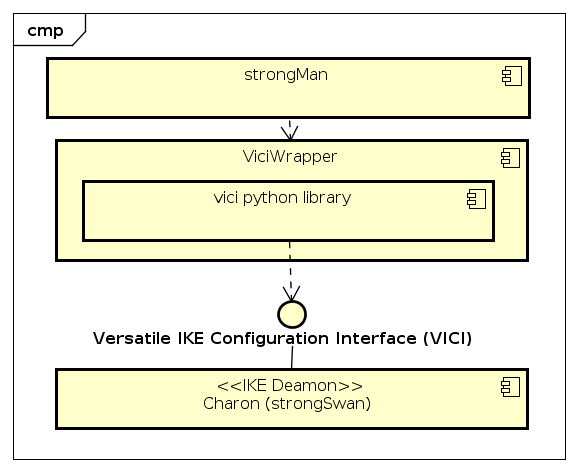
\includegraphics[width=250pt]{images/vici_wrapper.png}
\caption[Vici Diagramm]{Vici Diagramm}
\end{figure}
\medskip
Die Kommunikation, welche durch die Schnittstelle angeboten wird, basiert auf einem Unix Socket (AF\_UNIX). Dabei wird in Python die OrderedDictionary-Klasse verwendet, die als verschachtelte Property List für die Konfigurationsparameter dient. \footnote{\url{https://github.com/strongswan/strongswan/tree/master/src/libcharon/plugins/vici}}\\

\begin{python}
OrderedDict([
	('cert', OrderedDict([
		('remote_addrs', ['gateway'])
	)])
])
\end{python}

\newpage
\subsection{Log Messages}
\subsubsection{Ausgangslage}
Eine VPN Tunnel wurde mit Hilfe des strongMan korrekt konfiguriert und steht nun bereit für den Auf- und Abbau.
Der Tunnel wird gestartet, dies lösst auf der Client Seite einen Asynchronen Request aus, der auf dem Backend die Daten des konfigurierten Tunnels aus der Datenbank liest und in eine passende Form für die VICI Schnittstelle aufbereiten und übergibt. Die geladene Verbindung wird nun gestartet, was zur Folge hat, dass blockierend ein Generator zurück gegeben wird. Welcher jede neue Nachricht in die Datenbank loggt.

\subsubsection{Problematik}
Die Log Nachrichten werden durch einen Thread, dessen Laufzeit nicht bekannt ist, mit Hilfe des Generators in die Datenbank geschrieben. Der Thread terminiert, wenn ein Tunnel aufgebaut wurde oder falls dies nicht möglich war erst nach mehreren Retry versuchen. Während dieser Zeit werden diverse Logs gespeichert, die dem Benutzer möglichst in Echtzeit angezeigt werden sollten. 

\subsubsection{Lösungsansatz}
Das laden der Connection Overview Seite lösst einen Long Polling Request aus, der alle zuest alle Logs die älter als 5 Minuten sind aus der Datenbank löscht und die restlichen dem Frontend zurück gibt. Die führt dazu , dass ein neuer Long Polling Request gestartet wird, welcher den neusten Log als Parameter mit gibt und nun nur noch neuere Meldungen übermittelt werden. Dies wird wiederholt, bis die Connection Overview Seite verlassen wird.
\medskip
\begin{figure}[H]
\centering
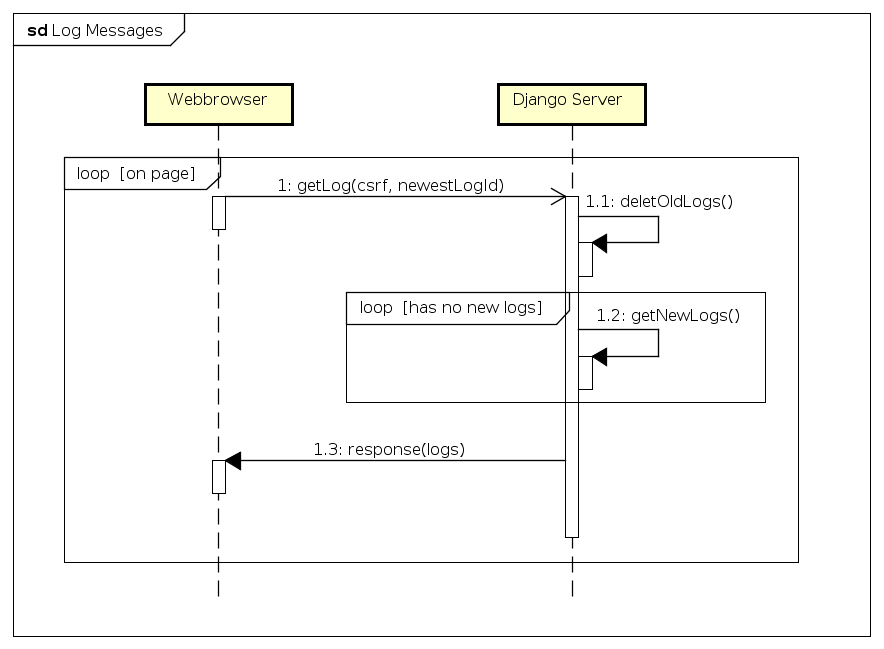
\includegraphics[width=400pt]{images/log_messages_seq.png}
\caption[Log Messages Sequenzdiagramm]{Log Messages Sequenzdiagramm}
\end{figure}
\subsection{Subklassen}
\subsubsection{Ausgangslage}
Um die diversen Authentiserungsmethoden sowohl in der Datenbank, wie auch in unseren Models widerzuspiegeln, setzen wir auf Vererbung. Wird in Django Vererbung beim Models eingesetzt wird standardmässig "Multi-table inheritance" verwendet, dass heisst es gibt für jede Subklasse eine weiter Tabelle in der Datenbank.

\subsubsection{Beispiel Vererbung}
Beispiel Code in Django um die Vererbung zu demonstrieren.
\medskip
\begin{python}
from django.db import models

class Authentication(models.Model):
    name = models.TextField()
    round = models.IntegerField(default=1)

class EapAuthentication(Authentication):
    eap_id = models.TextField()
\end{python}

\medskip
Dies führt zu folgenden Tabellen in der Datenbank:
\medskip

\begin{table}[H]
	\centering
    \begin{tabular}{|p{3cm}|p{3cm}|p{3cm}|}
    \hline    
    \rowcolor{lightblue}
	id & name & round \\ \hline   
	1 & eap home & 1 \\ \hline
	2 & cert work & 1 \\ \hline
    \end{tabular}
    \caption[Authentication]{Authentication}
\end{table}
\medskip \medskip
\begin{table}[H]
	\centering
    \begin{tabular}{|p{4.5cm}|p{4.5cm}|}
    \hline    
    \rowcolor{lightblue}
	authentication\_ptr\_id & eap\_id \\ \hline   
	1 & eap-home-id  \\ \hline
    \end{tabular}
    \caption[EapAuthentication]{EapAuthentication}
\end{table}
\medskip

\subsubsection{Problematik}
Nun wird bei Request vom Frontend an das Backend oft nur die \textbf{id} des Models übermittelt.\\
Dies könnte wie folgt aussehen:
\medskip
\begin{python}
def update(request, id):
    authentication = Authentication.objects.get(id=id)
    ...
\end{python}
\medskip
Wie erwartet ist das Objekt \textbf{authentication} vom Typ Authentication. Falls hinter dieser \textbf{id} jedoch noch eine Spezialisierung stecken würde, sieht man dies dem Objekt nicht an.
\subsubsection{Lösungsansatz}
Die Lösung für dieses Problem bietet Django selbst leider nicht an. Jedoch ist eine elegante Möglichkeit die Spezialisierung des Objektes über Reflection zu lösen. Dazu implementieren wir in den Basisklassen die Methode \textbf{subclass()}.\\
Diese ermöglicht es für jede Subklasse der Basisklasse zu testen, ob das aktuelle Objekt eine Spezialisierung ist oder nicht, falls ja, wird ein neue spezialisierte Instanz erstellt und zurück gegeben.
\medskip
\begin{python}
class Authentication(models.Model):
	...
	
    @classmethod
    def get_types(cls):
        subclasses = [subclass() for subclass in cls.__subclasses__()]
        return [subclass.get_typ() for subclass in subclasses]	
	
    def subclass(self):
        for cls in self.get_types():
            authentication_class = getattr(sys.modules[__name__], cls)
            authentication = authentication_class.objects.filter(id=self.id)
            if authentication:
                return authentication.first()
        return self
\end{python}
\medskip
Mit Hilfe dieser Erweiterung sieht das verbesserte obig Beispiel nun folgendermassen aus.
\medskip
\begin{python}
def update(request, id):
    authentication = Authentication.objects.get(id=id).subclass()
    ...
\end{python}
\medskip
Der Typ des \textbf{authentication} Objektes entspricht nun der gewünschten Subklasse.

\newpage
\subsection{Verschlüsselte Datenbankfelder}
Während des Projekts ist die Anforderung von der Verschlüsslung der Datenbank aufgekommen. Die Datenbank verfügt über sensible Daten wie Private Keys und Passwörter, die nicht einfach offen gelesen werden dürfen.\\


\decision{Datenbankfelder werden mit einem Secret Key verschlüsselt}
Nach einer Besprechung mit unserem Betreuer, haben wir uns auf die Verschlüsslung von einzelnen sensiblen Datenbankfelder mit einem Secret Key entschieden. Der Secret Key muss bei jeder Neuinstallation der Applikation zufällig generiert werden.\\


Das Projekt  Django Fernet-Fields\footnote{\url{https://github.com/orcasgit/django-fernet-fields}} stellt ein angepasstes Datenbankfeld EncryptedField zur Verfügung, das als Django ORM Feld verwendet werden kann. Django kann Klartext in EncryptedField schreiben und wieder Klartext daraus lesen. EncryptedField übernimmt das ganze Verschlüsslungsmanagement. In der Datenbank sind nur kryptische Zeichen zu finden.

\subsubsection{Anpassung des Fernet-Fields}
Das Fernet-Field Projekt benötigt die Python Bibliothek Cryptography\footnote{\url{https://cryptography.io/en/latest/fernet/}}, welche wiederum C++ Code während der Installation kompilieren muss. Um dies zu vermeiden und um die Installation zu vereinfachen, haben wir die EncryptedField Klasse leicht angepasst, damit diese pyaes\footnote{\url{https://github.com/ricmoo/pyaes}} nutzt und wir die Abhängigkeit zur Cryptography verlieren.

Beim ersten Start von strongMan generiert base.py einen neuen Secret Key\footnote{https://gist.github.com/ndarville/3452907} und schreibt diesen in die Datei db\_key.txt.
EncryptedField benutzt diesen Secret Key und verschlüsselt die Daten mit AES256.
\subsection{Zertifikate}
Um IPsec Verbindungen mit asymmetrischen Schlüsseln zu erstellen, müssen Schlüssel verwaltet werden. strongMan persistiert die geuploadeten Schlüsselcontainer in der Datenbank.
Dabei werden folgende Schlüsselcontainer Formate unterstützt: \\

\begin{tabular}{ | p{0.2\textwidth} | p{0.7\textwidth} | }
\hline
    Schlüsselcontainer: & X509, PKCS1, PKCS8, PKCS12 \\ \hline
    Encoding: & PEM, DER \\ \hline
    Algorithmen: & RSA, ECDSA \\ \hline
\end{tabular}
\\\\
Die Applikation hat ein Uploadfeld um Schlüsselcontainer hinzuzufügen. Dabei müssen die vier verschiedenen Containertypen unterschieden werden, um die Daten richtig auszulesen. Die Klasse ContainerDetector probiert die Datei mit allen vier ASN1 Strukturen zu parsen und gibt bei Erfolg den entsprechenden Typ zurück.

\subsubsection{Wichtige Implementationsmerkmale}
\paragraph{Private Keys} Wie im Domain Model zu erkennen ist, hängt der Private Key immer an einem UserCertificate. Das Zertifikat muss somit immer vor dem Private Key geuploadet werden. Dies verhindert Private Key Leichen in der Datenbank und vereinfacht das Schlüsselhandling.

\paragraph{Doppelte Einträge} Der CName ist normalerweise ein einfacher Eintrag wie www.raiffeisen.ch. In Ausnahmefällen kann der CName - oder auch andere Felder - auch eine Liste wie ['raiffeisen.ch', 'www.raiffeisen.ch'] sein. Die Liste wird in einen String umgewandelt und so dargestellt.

\paragraph{Doppelte Zertifikate/Private Keys}
Werden bestehende Zertifikate oder Private Keys nochmals geuploadet, erkennt die Zertifikatsverwaltung dies und verweigert den Upload. Das Matching wird anhand des Public Keys vorgenommen. Bei Zertifikaten wird der Public Key und die Version gematcht.

\paragraph{Zertifikate in Gebrauch}
Ist ein Zertifikat in einer Konfiguration ausgewählt, so kann das Zertifikat nicht gelöscht werden. Das Zertifikat muss zuerst deselektiert werden, um es aus der Zertifikatsverwaltung zu löschen.






\section{Testing}
In der Python Standard Library gibt es das Unit Testing Framework \textbf{unittest}, das erlaubt Unit Tests zu implementieren. 
Django's Unit Tests basieren auf dieser Library und erweitern diese, beispielsweise erbt \textbf{django.test.TestCase} von \textbf{unittest.TestCase}. Weiter werden auch Integrationtests ermöglicht.

\subsubsection{Beispiel Integrationtests}
\begin{python}
from django.test import Client, TestCase
from django.contrib.auth.models import User

class AboutViewsTests(TestCase):

   def setUp(self):
       self.user = User.objects.create(username='testuser')
       self.user.set_password('12345')
       self.user.save()
       self.client = Client()
       self.client.login(username='testuser', password='12345')

   def test_about_get(self):
       response = self.client.get('/about/')
       self.assertEquals(response.status_code, 200)      
\end{python}

\subsection{Continuous Integration (CI)}
Der Aufbau der Continuous Integration Umgebung des strongMans ist nicht trivial und stellt folgede Anforderungen:
\begin{itemize}
	\item Aufbau von IPsec Tunnels zwischen mindesten zwei Rechnern
	\item automatisierter Ablauf
	\item geringe Einarbeitungszeit in Technologien
	\item möglichst kostenfreie Dienste nutzen
\end{itemize}
Um den Anforderungen gerecht zu werden setzten wir auf ein Zusammenspiel folgender Tools:
\paragraph{GitHub} wird von uns als online Repository verwendet und wird mit dem Versionsverwaltungssystem Git eingesetzt. Weiter bietet es für andere Dienste WebHooks an. 
\paragraph{Travis CI} wird als eigentlicher Continuous Integration Anbieter verwendet. Es ermöglicht automatisierte Builds und Tests. Travis CI ist für Projekte, welche auf GitHub gehostet werden, ausgelegt.

\paragraph{Docker} Um die strongSwan Konfiguration direkt zu testen, wird docker-compose eingesetzt. Docker-compose gewährleistet mehrere Docker Container zu builden, ein Netzwerk untereinander und somit einen IPsec Tunnel aufzubauen. \\

\subsubsection{Ablauf}
\begin{figure}[H]
\centering
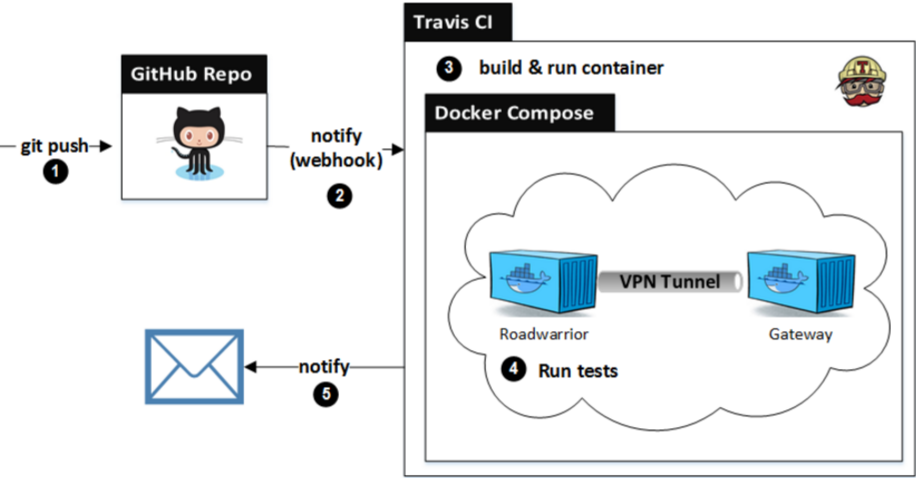
\includegraphics[width=420pt]{images/testing.png}
\caption[Schematische Darstellung der Testumgebung]{Schematische Darstellung der Testumgebung}
\end{figure}\medskip
\begin{enumerate}
	\item git push, lokaler Code wird auf GitHub publiziert.
	\item Travis CI wird durch WebHook notifiziert.
	\item Travis CI buildet zwei Docker Container, welche auf der Basis des offiziellen Django Container aufbaut.
	\begin{enumerate}
         \item StrongSwan mit den nötigen Plugins wird installiert und gestartet.
         \item Auf dem Roadwarrior wird die strongMan Applikation vom GitHub Repository installiert und der aktuelle Branch wird eingecheckt.
      \end{enumerate}
      \item Der Roadwarrior started die Unit- und die Integrationstests. Dabei werden zwischen den Docker Container diverse Ipsec Tunnels auf- und abgebaut.
      \item Erfolg und Misserfolg ist auf der ReadMe Seite auf Github einsehbar.
\end{enumerate}

\newpage
\subsection{Usability Tests}

Die Usability Tests sollen Ablauffehler aufzeigen und die Benutzbarkeit der Applikation insgesamt steigern. Dazu sind in einer ersten Phase zwei Personas erstellt worden.
\\
\decision{Usability Tests vs. Server Features}
\label{UsabilityEntscheid}
Am Ende der zweit letzten Construction Phase, nach einer Besprechung mit Herrn Steffen, entschieden wir uns Usability Tests durchzuführen und den Server Teil der Applikation in diesem Projekt nicht zu implementieren.
Damit werden die Use Cases UC03: Child\_SA beenden und UC06: Admin Mode wechseln hinfällig.

\subsubsection{Primäre Persona User}





\noindent\begin{minipage}[t]{0.5\textwidth}
\vspace{0pt}
    \begin{tabular}{ l l }
        Name: & Markus Egger \\
        Alter: & 40 Jahre \\
        Beruf: & Verkäufer Aussendienst \\
        Wohnort: & Uster ZH \\
        Zivilstand: & Verheiratet, 2 Kinder \\
        Hobbies: & Gleitschirm, Bowling \\
        Sprachen: & Deutsch / Englisch \\
    \end{tabular}
\end{minipage}
\hfill
\begin{minipage}[t]{0.5\textwidth}
\vspace{0pt}

\begin{figure}[H]
\centering
    
\includegraphics[width=230px]{images/persona_business.jpg}
    \caption[Primäre Persona User]{Primäre Persona User}
\end{figure}
\end{minipage}
\medskip


Markus Egger arbeitet in einem mittelgrossen Industrieunternehmen und verkauft dort Isolationsmatten aus Steinwolle. Da er viel auf Reisen bei seinen Kunden ist und dadurch längere Zeit keinen physischen Zugang zum Firmennetzwerk hat, benutzt er eine VPN Software um auf firmeninterne Daten zuzugreifen. Seine Informatikfähigkeiten beziehen sich dabei auf die in seiner KV Lehre erworbenen Kenntnisse mit Email, Word und Excel, sowie dem oberflächlichen Umgang mit ERP/CRM Systemen.
Markus beherrscht die englische Sprache auf Verhandlungsniveau.

Zusätzlich zu seinen Reisen arbeitet Markus gerne auch mal Zuhause, um mehr Zeit bei seinen erst kürzlich eingeschulten Kindern zu verbringen und seine Frau zu entlasten.

\subsubsection{Test Vorlage}


Sie sind Angestellter in der Personalabteilung der Industriefirma Techtronic AG und arbeiten heute zum ersten Mal Zuhause an ihrem Arbeitslaptop. Um Zugriff auf firmeninterne Dokumente zur erhalten, müssen Sie eine sichere Verbindung zur Tectronic AG aufbauen. Dazu hat Ihnen die Informatikabteilung ein USB-Stick mit Anleitungen, Username, Passwort und Zertifikatsdateien zur Verfügung gestellt. Ihre Aufgabe ist es nun, die unten aufgeführten Tasks zu lösen.

\paragraph{Passwort ändern}
Loggen Sie sich ein und ändern Sie ihr Passwort. \\


\begin{tabular}{ | p{0.14\textwidth} | p{0.77\textwidth} | }
\hline
Preconditions: & Applikation ist gestartet. User befindet sich auf der Login Seite. \\
\hline
Hilfsmittel: & Username und aktuelles Passwort \\
\hline
Artefakte: & User konnte sich einloggen. \\ 
& Passwort ändern Feld gefunden. \\
& Passwort konnte geändert werden. \\
\hline
\end{tabular}

\paragraph{Verbindung erstellen}
Erstellen Sie eine neue Verbindung zur HSR mit den gegebenen Daten. \\


\begin{tabular}{ | p{0.14\textwidth} | p{0.77\textwidth} | }
\hline
Preconditions: & User befindet sich eingeloggt auf der Startseite von strongMan. Connections und Certificates sind leer. Der System Administrator hat eine Anleitung zum Erstellen der Verbindung zur Verfügung gestellt. \\
\hline
Hilfsmittel: & Schritt für Schritt Anleitung mit Server, Username, Passwort, CA-Zertifikat, Identity \\
\hline
Artefakte: & User hat den Connections Bereich gefunden. \\
& User hat den Add Button gefunden. \\
& Der richtige Authentifizierungstyp ist ausgewählt. \\
& Verbindung richtig ausgefüllt und erstellt. \\
\hline
\end{tabular}


\paragraph{Verbindung starten / stoppen}
Starten Sie die Verbindung und stoppen Sie diese wieder. \\


\begin{tabular}{ | p{0.14\textwidth} | p{0.77\textwidth} | }
\hline
Preconditions: & User befindet sich auf der Connections Seite. Die in Aufgabe 2 erstellte Connection ist abgespeichert. \\
\hline
Hilfsmittel: & - \\
\hline
Artefakte: & User erkennt den On/Off Button. \\
& User kann die Verbindung starten. \\
& User ist sich bewusst, dass die Verbindung jetzt steht (Fragen!). \\
& Verbindung ist wieder gestoppt. \\
\hline
\end{tabular}

\newpage
\subsubsection{Sekundäre Persona Administrator}

\noindent\begin{minipage}[t]{0.5\textwidth}
\vspace{0pt}
    \begin{tabular}{ l l }
        Name: & Remo Stoop \\
        Alter: & 28 Jahre \\
        Beruf: & System Administrator \\
        Wohnort: & Greifensee ZH \\
        Zivilstand: & Konkubinat, 1 Kind \\
        Hobbies: & Raspberry Pi, Gamen \\
        Sprachen: & Deutsch / Englisch \\
    \end{tabular}
\end{minipage}
\hfill
\begin{minipage}[t]{0.5\textwidth}
\vspace{0pt}
\begin{figure}[H]
\centering
    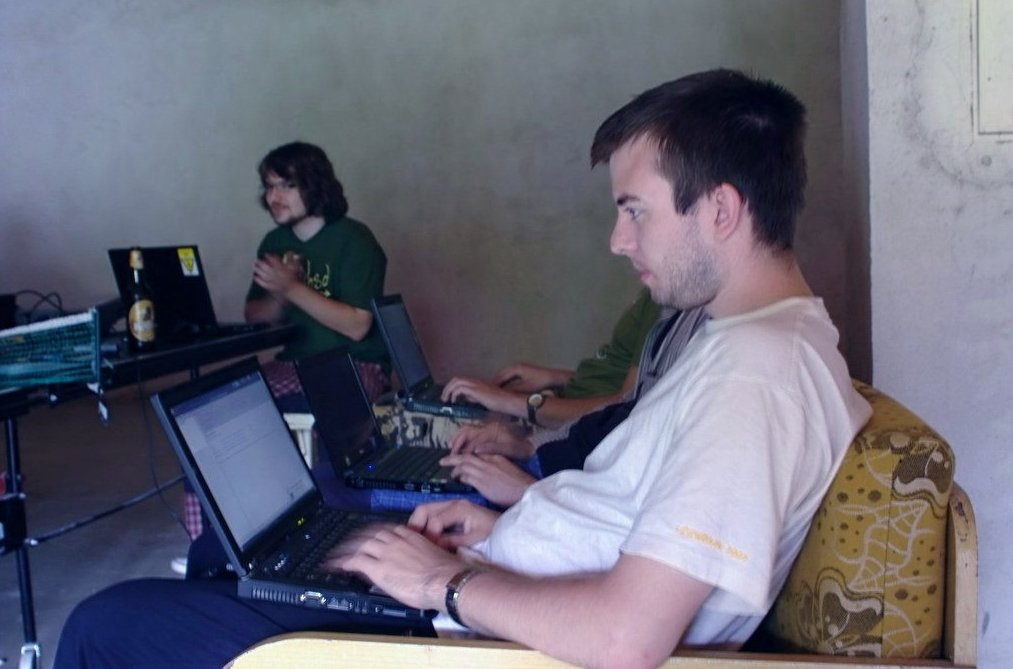
\includegraphics[width=230px]{images/administrator.jpg}
    \caption[Sekundäre Persona Administrator]{Sekundäre Persona Administrator}
\end{figure}
\end{minipage}
\medskip

Remo Stoop arbeitet wie Markus Egger im gleichen mittelgrossen Industrieunternehmen, welche Isolationsmatten herstellt. Er ist dort als System Administrator angestellt und verantwortlich für die Netzwerkinfrastruktur und der Netzwerksicherheit, inklusive dem Netzwerkzugriff von aussen.  Remo hat sich bewusst in Richtig Netzwerk weitergebildet. Nach seiner Lehre als Informatiker Systemtechnik hat er zwei fünf tägige Cisco Netzwerk Kurse besucht und ist seit dem netzwerktechnisch auf dem neusten Stand. Die symmetrischen und asymmetrischen Verschlüsslungstechniken kennt er oberflächlich aus einem Modul aus seiner Lehre.

Auch Remo arbeitet gerne einen Tag in der Woche zuhause, sofern es seine Arbeit erlaubt. Neben seiner Familie ist seine Hauptbeschäftigung das Gamen mit Freunden sowie Raspberry Pi Bastelprojekte.


\subsubsection{Test Vorlage (erweitert User Tests)}

Sie sind Systemadministrator der Industriefirma Techtronic AG und haben zuvor einen strongSwan VPN Server eingerichtet. Nun soll das erste Mal eine Verbindung von ausserhalb (genauer von Ihnen zuhause) in die Firma aufgebaut werden. Dazu stehen Ihnen Username, Passwort und Zertifikatsdateien zur Verfügung gestellt. Ihre Aufgabe ist es nun, die unten aufgeführten Tasks zu lösen.

\paragraph{Key Container hinzufügen}
\begin{enumerate}
    \item Fügen Sie in der Zertifikatsverwaltung einen verschlüsselten PKCS12 Container hinzu.
    \item Fügen Sie in der Zertifikatsverwaltung ein neues Zertifikat mit Private Key hinzu.
    \item Welche Email Adresse ist beim Zertifkat roadwarrior.hsr.ch eingetragen?
    \item Zertifkat roadwarrior.hsr.ch löschen.
\end{enumerate}


\begin{tabular}{ | p{0.14\textwidth} | p{0.77\textwidth} | }
\hline
Preconditions: & User befindet sich auf der Startseite von strongMan. \\
\hline
Hilfsmittel: & Roadwarrior PKCS12 Container mit Passwort, Zertifikat mit Private Key \\
\hline
Artefakte: & User hat den Add Button gefunden. \\
& User konnte den verschlüsselten PKCS12 Container hinzufügen. \\
& User konnte das Zertifikat hinzufügen. \\
& User konnte den Private Key hinzufügen. \\
& User findet Email-Adresse. \\
& User konnte Zertifikat löschen. \\
\hline
\end{tabular}


\subsubsection{Fazit}
Wir haben die Usability Tests mit vier Personen durchgeführt. Die Administrator Tests haben zwei unbeteiligte HSR Studenten durchgeführt und die User Tests zwei User mit Büroerfahrung.

Die wichtigsten Erkenntnisse aus den Tests sind:
\begin{itemize}
    \item Es braucht ein Text, der beschreibt, dass zuerst das Zertifikat und erst danach der Private Key geuploaded werden kann.
    \item Die State Spalte in der Connection Table ist nicht sortierbar.
    \item Der Verbindungstyp muss änderbar sein nach der Auswahl.
    \item Zertifikate müssen in der Verbindungskonfiguration hinzugefügt werden können.
    \item Beschriftung der Remove Buttons muss eindeutig sein. Private Key löscht keine Zertifikate.
    \item Verbindung darf nicht löschbar sein, wenn sie aktiv ist.
    \item Diverese Verbesserungen an der Englischen Sprache sind nötig.
    \item Die Anordnung der Buttons im Add-Certificate Formular verwirrt.
    \item About Pages zeigt keine Infos.
\end{itemize}

\section{Codestatistik}
\subsection{Test Coverage}
Test Coverage wurde mit \textbf{Pycharm} durchgeführt. \\

\begin{table}[H]
\centering
    \begin{tabular}{|p{6cm}|p{6cm}|}
    \hline    
    \rowcolor{lightblue}
	App & Coverage [\%] \\ \hline
	connections & 88 \\ \hline    
	certificates & 88 \\ \hline   
	vici & 88 \\ \hline  
	encryption & 94 \\ \hline  
	\rowcolor{lightblue}
	Durchschnitt &   90 \\ \hline
    \end{tabular}
    \caption[Test Coverage]{Test Coverage}
\end{table}

\subsection{Codezeilen}
Die Codezeilen wurden mit Hilfe von \textbf{CLOC} \cite{CLOC} ausgezählt. \\

\begin{table}[H]
\centering
    \begin{tabular}{|p{3cm} |p{3cm} |p{3cm} |}
    \hline    
    \rowcolor{lightblue}
	Sprache & Dateien & Zeilen  \\ \hline   
	Python & 68 & 5402 \\ \hline
    \end{tabular}
    \caption[Codezeilen]{Codezeilen}
\end{table}


\newpage
\section{Resultate}
\subsection{Management-Oberfläche für VPN Clients}
\noindent\begin{minipage}[t]{0.6\textwidth}
\vspace{0pt}
    \begin{figure}[H]
    	\centering
    	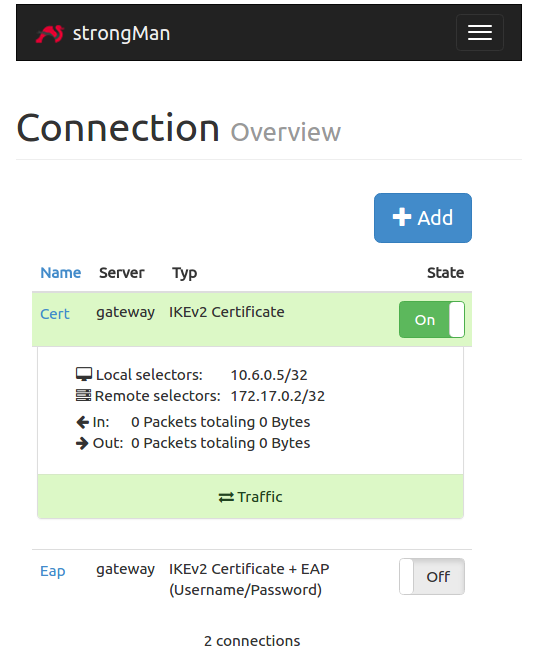
\includegraphics[width=250pt]{images/con_overview.png}
    	\caption{Connection Overview}
    \end{figure}
\end{minipage}
\hfill
\begin{minipage}[t]{0.4\textwidth}
\vspace{0pt}
Das ist die Connectin Overview.
\end{minipage}

\newpage

\subsection{Zertifikatsverwaltung}
\noindent\begin{minipage}[t]{0.4\textwidth}
\vspace{0pt}
Übersicht Zertifikatsverwaltung
\end{minipage}
\hfill
\begin{minipage}[t]{0.6\textwidth}
\vspace{0pt}
    \begin{figure}[H]
    	\centering
    	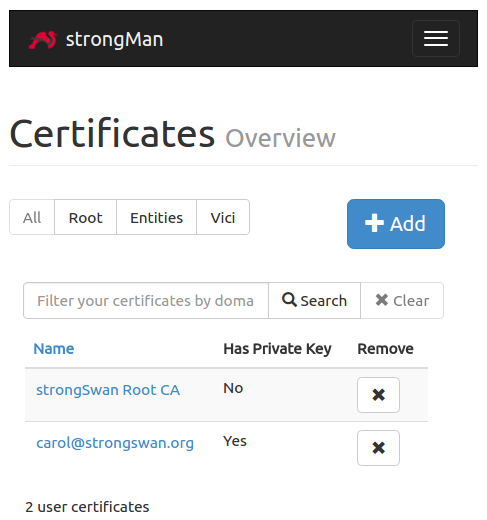
\includegraphics[width=250pt]{images/certificate_overview.png}
    	\caption{Certificate Overview}
    \end{figure}
\end{minipage}

\newpage
\chapter{Projektmanagement}
\newpage
\section{Rollen und Verantwortlichkeiten}

\subsubsection{Prof. Steffen Andreas}
\noindent\begin{minipage}{0.5\textwidth}
\begin{figure}[H]
	\centering
	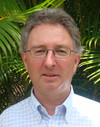
\includegraphics[height=30mm]{images/asteffen.jpg}
	\caption{Prof. Dr. Andreas Steffen}
\end{figure}
\end{minipage}
\hfill
\begin{minipage}{0.5\textwidth}
Professor, Institutsleiter ITA \\
\end{minipage}


\subsubsection{Tobias Brunner}
\noindent\begin{minipage}{0.5\textwidth}
\begin{figure}[H]
	\centering
	
\includegraphics[height=30mm]{images/unknown.png}
	\caption{Tobias Brunner}
\end{figure}
\end{minipage}
\hfill
\begin{minipage}{0.5\textwidth}
Institutsmitarbeiter ITA \\
\end{minipage}


\subsubsection{Bühler Severin}
\noindent\begin{minipage}{0.5\textwidth}
\begin{figure}[H]
	\centering
	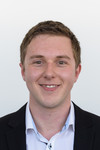
\includegraphics[height=30mm]{images/sbuehler.jpg}
	\caption{Bühler Severin}
\end{figure}
\end{minipage}
\hfill
\begin{minipage}{0.5\textwidth}
Severin Bühler, Student an der HSR, ist Entwickler des Projektes. \\
\end{minipage}

\subsubsection{Kurath Samuel}
\noindent\begin{minipage}{0.5\textwidth}
\begin{figure}[H]
	\centering
	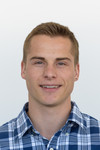
\includegraphics[height=30mm]{images/skurath.jpg}
	\caption{Kurath Samuel}
\end{figure}
\end{minipage}
\hfill
\begin{minipage}{0.5\textwidth}
Samuel Kurath, Student an der HSR, ist Entwickler des Projektes. \\
\end{minipage}
\section{Entwicklungsumgebung und Infrastruktur}
\subsubsection{IDE (Integrated Development Environment)}
\decision{PyCharm}	
Beiden Projektmitgliedern ist JetBrains Intellij bekannt und \Gls{PyCharm} ist im Umgang nahe zu identisch.
Für Studenten sind die Entwicklungsumgebungen kostenlos verfügbar.
\subsubsection{SCM (Source Control Management)}
\decision{GitHub}
Der Umgang mit \Gls{Git} ist beiden Projektmitglieder bestens bekannt.
\Gls{GitHub} ist ohne Unkosten von überall verfügbar.
Das Geometalab der HSR publiziert über diesen Weg diverse Projekte.

\subsubsection{CI (Continuous Integration)}
\decision{Travis CI}
Mit \Gls{Travis CI} wurde ein Anbieter gefunden, der die eher komplexeren Anforderungen an das automatisierte Testing des strongMan Projektes erfüllt, sich nathlos in Github integrieren lässt, kostenfrei ist, sowie den Projektmitgliedern schon bekannt ist.

\subsubsection{Projektmanagement Tool}
\decision{Jira}
\Gls{Jira} ist den Projektmitgliedern schon aus der Studienarbeit bekannt und hat sich sehr bewährt.
Das Dashboard ist übersichtlich gestaltet. Es ermöglicht eine Übersicht über die aktuellen Tasks auf einen Blick.
Alle Mitglieder haben jederzeit Zugriff auf die Plattform, was die Transparenz erhöht.
Weiter bietet Jira diverse Reports um Auswertungen über das Projekt zu fahren.

\section{Planung}
Das Projekt strongMan wird in einer Mischung aus \Gls{RUP} und Agile durchgeführt. Der Projektzeitraum wird zuerst in die RUP Phasen Inception, Elaboration, Construction und Transition aufgeteilt, wobei wir in der Construction agile vorgegangen wird.

\subsection{Phasen}
\begin{enumerate}
  \item Inception
  \begin{enumerate}
    \item Einarbeitung in das Projekt
  \end{enumerate}
  \item Elaboration1
  \begin{enumerate}
    \item Evaluation und Einarbeitung der Techniken (Django, Crypto-Library, Vici-Schnittstelle)
    \item Erstellen der Requirement-Analyse
  \end{enumerate}
  \item Construction1
  \begin{enumerate}
    \item VPN-Tunnel CRUD
    \item VPN-Tunnel starten/stoppen
    \item Login 
    \item Zertifikate CRUD
  \end{enumerate}
  \item Construction2
  \begin{enumerate}
    \item Bestehende Verbindung terminieren
    \item User Password änedern 
    \item Verbindungselemente zwischen VPN-Tunnel und Zertifikate
    \item Verschlüsslung Private Keys und User Password für Tunnels
  \end{enumerate}
    \item Construction3
  \begin{enumerate}
  	\item Erstellen einer Informationsseite
    \item Optional: Administrationsmodus um Serverkonfigurationen vor zu nehmen
  \end{enumerate}
      \item Construction4
  \begin{enumerate}
    \item Applikation finalisieren
    \item Deployment
  \end{enumerate}
  \item Transition
  \begin{enumerate}
    \item Dokumentationsabschluss
  \end{enumerate}
\end{enumerate}
\newpage







\begin{landscape}
	\begin{figure}[H]
		\centering
		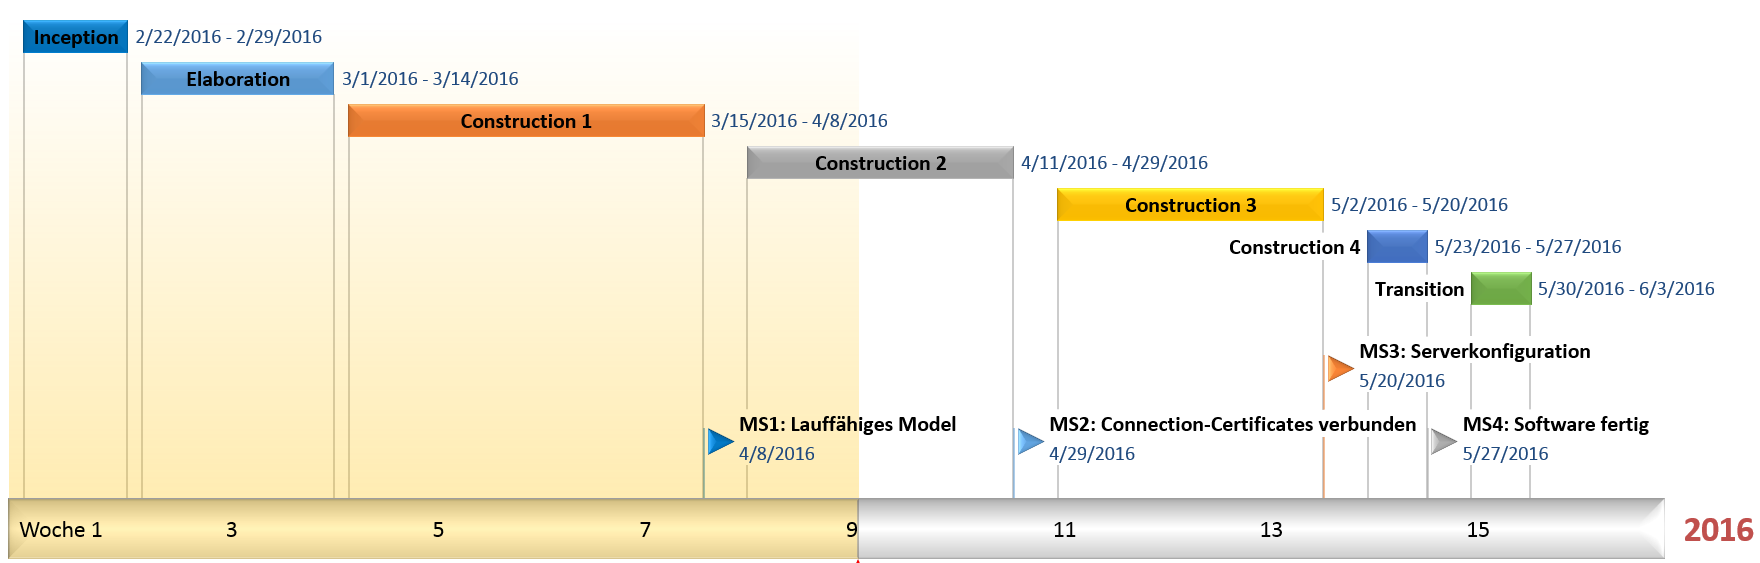
\includegraphics[width=250mm]{images/gantt.PNG}
		\caption{Gantt Chart}
	\end{figure}
\section{Risiken}
Um den Problemen, die während des Projekts auftreten können entgegenzuwirken, haben wir eine Risiko Analyse durchgeführt. Diese konnte dann bei der Planung eingesetzt werden.

\subsection{Technische Risiken}
\begin{table}[H]
    \begin{tabular}{|p{0.4cm}|p{2.5cm}|p{7cm}|p{1.5cm}|p{2.25cm}|p{1.75cm}|p{3cm}|p{4cm}|}
    \hline    
    \rowcolor{lightblue}
    Nr & Titel & Beschreibung & maximaler Schaden & Eintrittswahr-scheinlichkeit & Gewichteter Schaden & Vorbeugung & Verhalten beim Eintreten \\ \hline
	R1 & Python Crypto Library & Die evaluierte Crypto Library für die Zertifikaterkennung ist fehlerhaft oder ungenügend. & 50h & 20\% & 10h & Evaluation Library & Zertifikate werden nicht mehr ausgelesen, sondern nur noch stupid importiert. \\ \hline
	R2 & Komplexität VICI-Schnittstelle & Die Python Vici Schnittstelle deckt sich nicht mit der swanControl Notation. Dadurch kann massiv mehr Aufwand während der Implemenation entstehen. & 50h & 40\% & 20h & Die Vici Schnittstelle muss mit dem Prototypen gut durchgetestet werden, um Fehler möglichst früh zu finden. & Kontakt mit Tobias Brunner aufnehmen \\ \hline
	R3 & Einrichten automatisierte Testumgebung & Aufbau und Einrichten einer Integrationtestumgebung, welche es erlaubt Ipsec Tunnels zwischen mehreren Rechnern aufzubauen. & 60h & 60\% & 36h & Informationen zu CI Anbieter sammeln & Eigene Infrastruktur verwenden. \\ \hline
    \end{tabular}
    \caption[Risiken]{Risiken - Die technischen Risiken wurden zu Beginn des Projektes, wie in der Tabelle ersichtlich, definiert.}
\end{table}
\end{landscape}

\subsection{Auswertung}
\paragraph{R1 Python Crypto Library} Mit Hilfe der Evaluation der Crypto Library konnte dieses Risiko aus dem Weg geräumt werden. Der Aufwand blieb im erwarteten Rahmen und mit \textbf{oscrypto} wurde eine passende pure Python Bibliothek gefunden werden.

\paragraph{R2 Komplexität VICI-Schnittstelle} Das Zusammenspiel zwischen Pyhton/Django funktionierte nahtlos und wie in der Dokumentation beschrieben. Problematischer und Zeitintensiver war jedoch das korrekte Konfigurieren von strongSwan. Die 

\paragraph{R3 Einrichten automatisierte Testumgebung}
Docker-compose legte die Grundsteine, welche es uns ermöglichten mehrere Rechner für die Testumgebung zu nutzen. Da der uns wohl bekannte CI Anbieter Travis dies zudem noch unterstützt wurden automatische Integrationtest möglich. Das Finden einer passenden Lösung war ohne grössere Komplikationen möglich. Mehr Aufwand als erwartet, gab jedoch die Konfiguration der Docker-Container. Womit dieses Risiko teils eintrat.\\
\medskip
\begin{table}[H]
	\centering
    \begin{tabular}{|p{2cm}|l|p{2cm}|}
    \hline    
    \rowcolor{lightblue}
	Nr & Titel & Schaden \\ \hline   
	R1 & Python Crypto Library & 0h \\ \hline
	R2 & Komplexität VICI-Schnittstelle & 0h \\ \hline
	R3 & Einrichten automatisierte Testumgebung& 0h \\ \hline
	\rowcolor{lightblue}
	Total &  & 0h \\ \hline
    \end{tabular}
    \caption[Risikoauswertung]{Risikoauswertung}
\end{table}

\section{Arbeitsaufwand}
\subsubsection{Soll}

\begin{table}[H]
	\centering
    \begin{tabular}{|p{6cm}|p{6cm}|}
    \hline    
    \rowcolor{lightblue}
	Phase & Aufwand \\ \hline   
	Inception & 1 Woche \\ \hline
	Elaboration & 2 Wochen \\ \hline
	Construction1 & 3 Wochen \\ \hline
	Construction2 & 3 Wochen \\ \hline
	Construction3 & 3 Wochen \\ \hline
	Construction4 & 3 Wochen \\ \hline
	Transition & 1 Woche \\ \hline
	\rowcolor{lightblue}
	Total & 14 Wochen \\ \hline
    \end{tabular}
    \caption[Zeitplanung]{Zeitplanung}
\end{table}
\medskip
Um den Aufwand über die ganze Projektdauer ausgeglichen zu verteilen rechneten wir mit:
\begin{itemize}
    \item Aufwand pro Woche: 52 Stunden
    \item Aufwand geplant Total: 52 Stunden * 14 Wochen = \textbf{728 Stunden}
    \item Aufwand pro Student: 728 Stunden / 2 = \textbf{364 Stunden}
\end{itemize}

Das Frühlingssemester 2016 an der HSR hat offiziell 15 Wochen  (inklusive Ostern, Auffahrt und Pfingsten). Bis zur Abgabe der Bachelorarbeit, dem 18.06.2016, sind zusätzlich zwei weitere Wochen gegeben. Damit am Ende es Projektes der Aufwand nicht exponentiell steigt, planten wir unsere Stunden über das offizielle Frühlingssemester und hielten uns die restliche Zeit als Reserve frei.
\newpage
\subsubsection{Ist}
Während des ganzen Projektes haben wir in Jira Phasen geplant, dazu Tasks erstellt und entsprechen Zeit verbucht.

\begin{figure}[H]
	\centering
	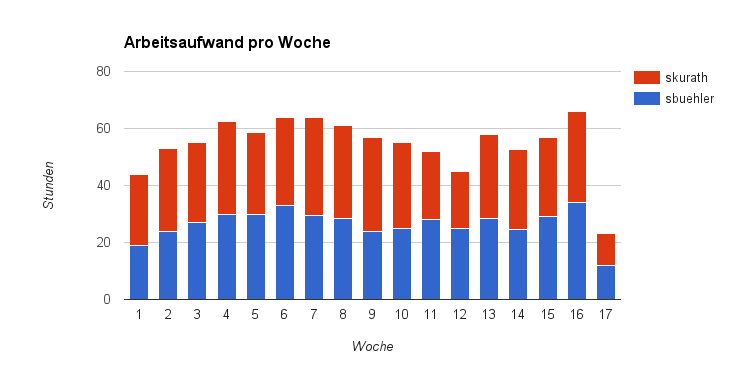
\includegraphics[width=480pt]{images/arbeitsaufwand.png}
	\caption{Arbeitsaufwand pro Woche}
\end{figure}

\begin{table}[H]
	\centering
    \begin{tabular}{|p{6cm}|p{6cm}|}
    \hline    
    \rowcolor{lightblue}
	Student & Aufwand \\ \hline   
	Severin Bühler & 451 Stunden \\ \hline
	Samuel Kurath & 476.5 Stunden \\ \hline
	\rowcolor{lightblue}
	Total & 927.5 Stunden \\ \hline
    \end{tabular}
    \caption[Arbeitsaufwand]{Arbeitsaufwand}
\end{table}

\newpage
\section{Erfahrungsbericht}
\subsubsection{Samuel Kurath}
Das Projekt strongMan war einen ausgezeichnete Gelegenheit die während dem Studium erlangten Software Engineering Kenntnisse umzusetzen. Mit der Verwendung einer Automatisierten Testumgebung und natürlich den implementierten Unit- wie auch Integrationtests konnten auch grössere Änderungen am Code vorgenommen werden ohne später auf unerwünschte Fehler zu stossen.\\
Weiter hatten wir die Gelegenheit unser Wissen in diversen Technologien auszubauen, dazu zähle ich Pyhton, Schlüsselcontainer und Docker. Auch neues wurde erlernt, mit Django einem Pyhton basiertem Webframework und der Docker Erweiterung docker-compose konnte mein persönlicher Toolstack bereichert werden.\\
Die Arbeit am strongMan und die Zusammenarbeit im Team, sowie die Betreuung durch den Experten war immer sehr harmonisch und produktive, was sich aus meiner Sicht auf das positive gelingen des Projektes ausgewirkt hat.


\subsubsection{Severin Bühler}
Während dieses Projekts kamen sehr viel neue oder nur in der Theorie bekannte Technologien wie Django, VirtualEnv, asymmetrische Schlüsselcontainer, SystemD, Webserver auf mich zu. Die Einarbeit in diese war sehr spannend und ich haben einiges gelernt. Auch die vertiefte Arbeit mit Python selbst mich noch einige weitere sprachspezifische Eigenheiten lernen lassen.

Nicht desto trotz hatte die Verwendung von Django auch seine negativen Seiten. Das Django ORM hat einen schwerwiegenden Nachteil bezüglich Vererbung (siehe Seite \pageref{subklassen}) und wir hatten einige Mühe diesen zu umgehen. Auch das Django Templating hat seine mühsamen Seiten.

Die Zusammenarbeit mit Herrn Steffen und auch Herr Brunner war auch zu jedem Zeitpunkt zielorientiert und positiv. Bei Fragen konnten wir immer auf die Unterstützung von ihnen zählen und wir standen nie unter überzogenem Leistungsdruck. 



\newpage
\chapter{Softwaredokumentation}
\newpage
\section{setup.py}
Die Datei 'setup.py' im Hauptverzeichnis des Projekts stellt das Installationsskript für strongMan dar. Zusätzlich enthält es noch einen migrate Befehl für das automatische Migrieren der Datenbank.

\begin{lstlisting}[style=BashInputStyle]
	 ./setup.py <command> [options]
\end{lstlisting}

\begin{itemize}
	\item -v | --verbose
	\begin{itemize}
	    \item Setzt die Ausgabe von setup.py auf verbose.
	\end{itemize}
\end{itemize}

\subsubsection{install}
\begin{lstlisting}[style=BashInputStyle]
	 ./setup.py install [-p %python-interpreter%]
\end{lstlisting}
Macht strongMan bereit zur Ausführung. Richtet ein Python Virtualenv ein, installiert alle Requirements, migriert die Datenbank und kopiert alle statischen Dateien in einen Ordner.
\begin{itemize}
	\item -p | --python %python-interpreter%
	\begin{itemize}
	    \item Wähle einen spezifischen Python Interpreter für strongMan
	    \item Python3 wird als Standartwert genutzt, wenn nichts angegeben.
	\end{itemize}
\end{itemize}

\subsubsection{uninstall}
\begin{lstlisting}[style=BashInputStyle]
	 ./setup.py uninstall
\end{lstlisting}
Versetzt die strongMan Applikation in den gleichen Zustand wie vor der Installation. Entfernt das Virtualenv und löscht die statischen Dateien.

\subsubsection{add-service}
\begin{lstlisting}[style=BashInputStyle]
	 sudo ./setup.py add-service
\end{lstlisting}
Fügt einen Systemd service für strongMan hinzu. Der Service ist zu Beginn gestoppt und disabled.\\

Starte den Service mit folgendem Befehl:
\begin{lstlisting}[style=BashInputStyle]
	 sudo systemctl start strongMan.service
\end{lstlisting}

Lasse den Service automatisch starten beim Systemstart:
\begin{lstlisting}[style=BashInputStyle]
	 sudo systemctl enable strongMan.service
\end{lstlisting}
Es werden Root Rechte benötigt, um Änderungen am Systemd zu machen.

\subsubsection{remove-service}
\begin{lstlisting}[style=BashInputStyle]
	 sudo ./setup.py remove-service
\end{lstlisting}
Entfernt den Systemd Service.

\subsubsection{migrate}
\begin{lstlisting}[style=BashInputStyle]
	 ./setup.py migrate [-dm]
\end{lstlisting}
Migriert die Django Datenbank, wenn Änderungen vorhanden sind. Siehe Django Migrations\footnote{\url{https://github.com/strongswan/strongswan/tree/master/src/libcharon/plugins/vici}}.
\begin{itemize}
	\item -dm | --delete-migrations
	\begin{itemize}
	    \item Löscht alle alten Migrationsskripte und die Sqlite Datenbank.
	\end{itemize}
\end{itemize}
\section{Benutzerhandbuch}

\section{Installation}
\subsubsection{Anforderungen}
\begin{itemize}
	\item strongSwan mit Vici plugin (>= v5.4.0)
	\item python3 =<
	\item pip3 =<
	\item git
	\item virtualenv
\end{itemize}
\subsubsection{Installation}
\begin{lstlisting}[style=BashInputStyle]
	 git clone https://github.com/Sebubu/strongMan.git
	 cd strongMan
	 ./setup.py install
\end{lstlisting}

\subsubsection{Starten}
\begin{lstlisting}[style=BashInputStyle]
	 ./run.py
\end{lstlisting}

\subsubsection{Systemd Service hinzufügen (Optional)}
Füge einen Systemd Service hinzu, der strongMan bei jedem Systemstart automatisch startet.
\begin{lstlisting}[style=BashInputStyle]
    sudo ./setup.py add-service # Adds the service
    sudo systemctl enable strongMan.service
    sudo systemctl start strongMan.service
\end{lstlisting}

\subsection{Deinstallation}
\subsubsection{Systemd Service entfernen (Optional)}
Entferne den Systemd Service, wenn installiert.
\begin{lstlisting}[style=BashInputStyle]
    sudo ./setup.py remove-service
\end{lstlisting}

\subsubsection{Entferne Programmordner}
Der Programmordner kann einfach gelöscht werden.
\begin{lstlisting}[style=BashInputStyle]
    rm -rf strongMan/
\end{lstlisting}



\newpage
\appendix
\newpage
\chapter{Mockups}
\label{Mockups}
\begin{figure}[H]
	\centering
	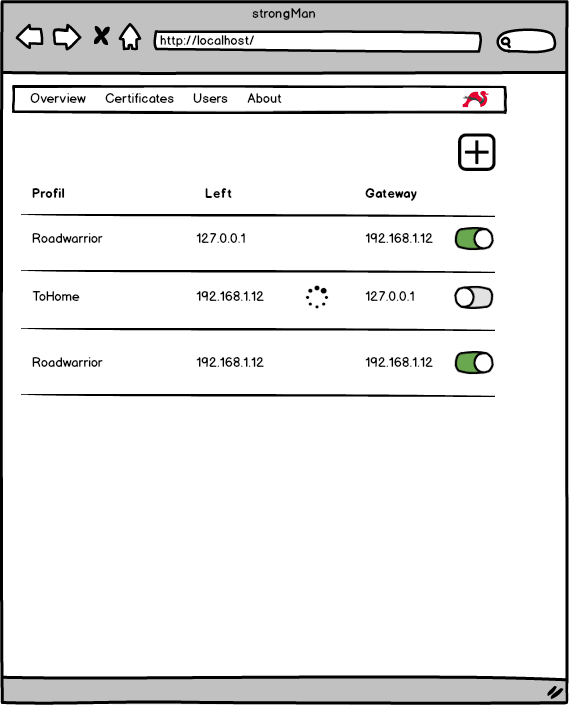
\includegraphics[width=400pt]{images/mockups/con_overview.png}
	\caption{Connection overview}
\end{figure}

\begin{figure}[H]
	\centering
	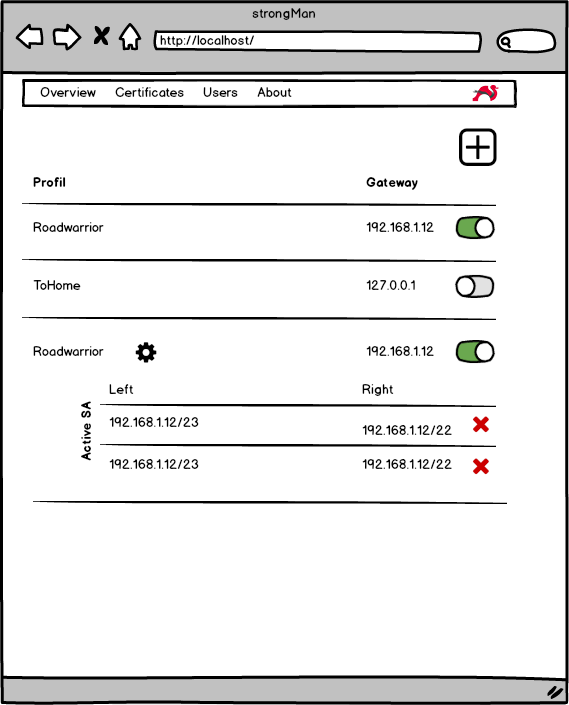
\includegraphics[width=400pt]{images/mockups/con_expanded.png}
	\caption{Connection overview - connected and expanded}
\end{figure}

\begin{figure}[H]
	\centering
	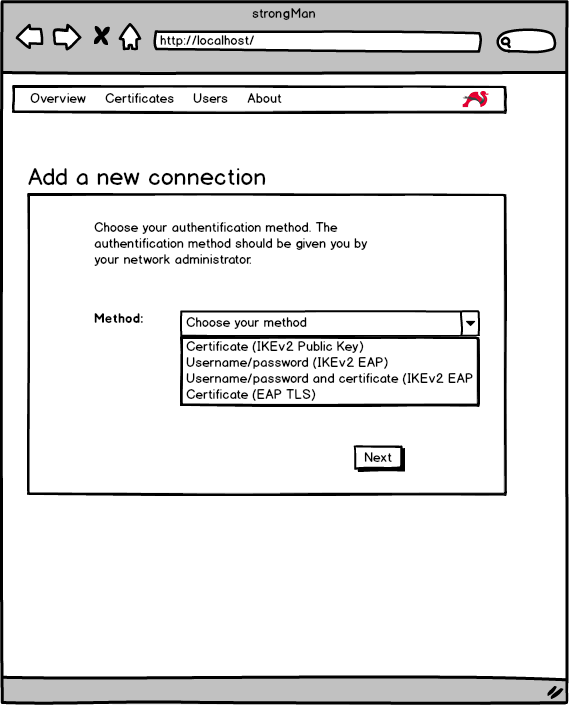
\includegraphics[width=400pt]{images/mockups/con_config1.png}
	\caption{Connection add - select method}
\end{figure}

\begin{figure}[H]
	\centering
	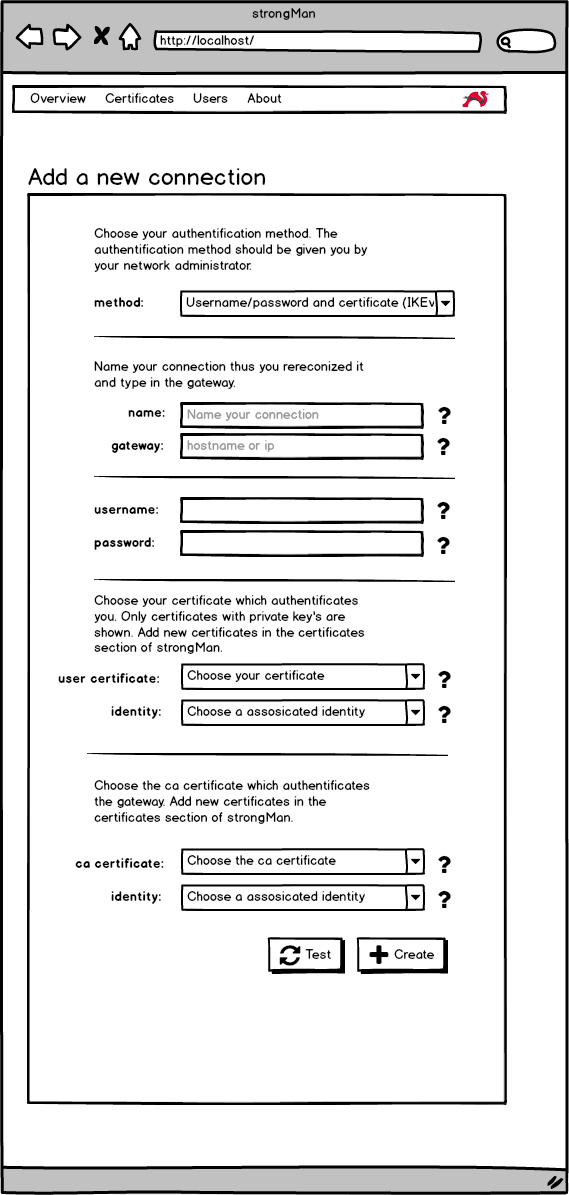
\includegraphics[width=350pt]{images/mockups/con_config2.png}
	\caption{Connection add - fill fields}
\end{figure}

\begin{figure}[H]
	\centering
	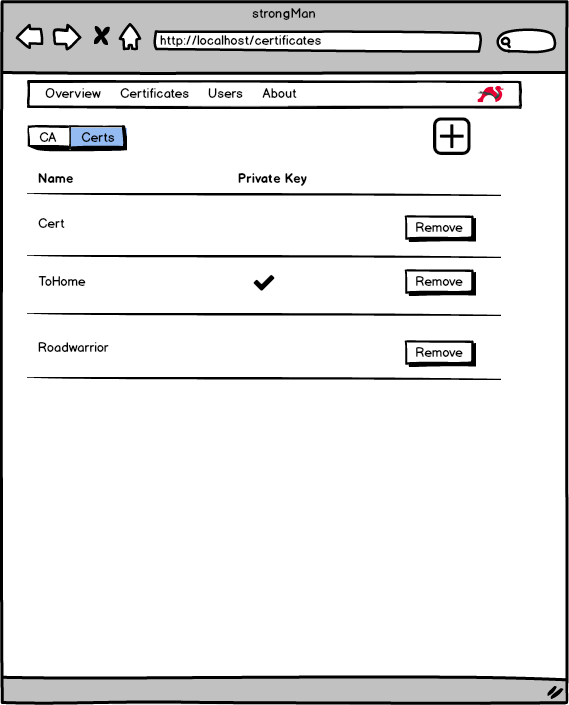
\includegraphics[width=400pt]{images/mockups/cert_overview1.png}
	\caption{Certificate overview}
\end{figure}

\begin{figure}[H]
	\centering
	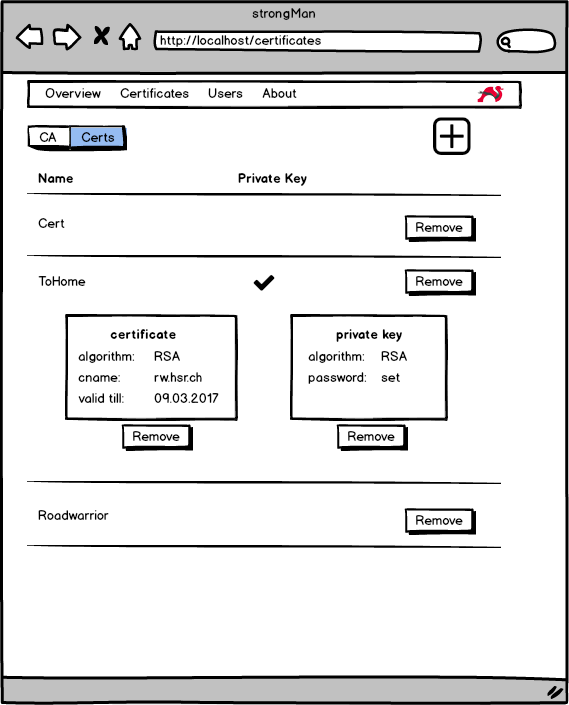
\includegraphics[width=400pt]{images/mockups/cert_overview_expanded2.png}
	\caption{Certificate overview - expanded}
\end{figure}

\begin{figure}[H]
	\centering
	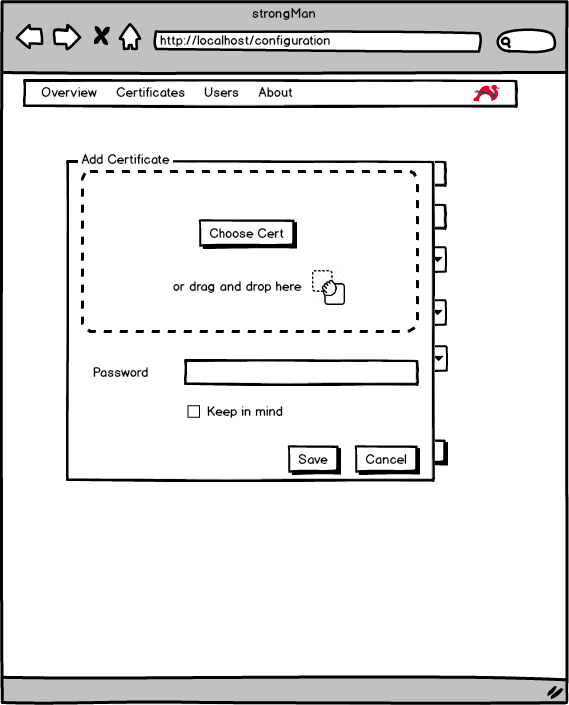
\includegraphics[width=400pt]{images/mockups/add_cert4.png}
	\caption{Add certificate}
\end{figure}

\begin{figure}[H]
	\centering
	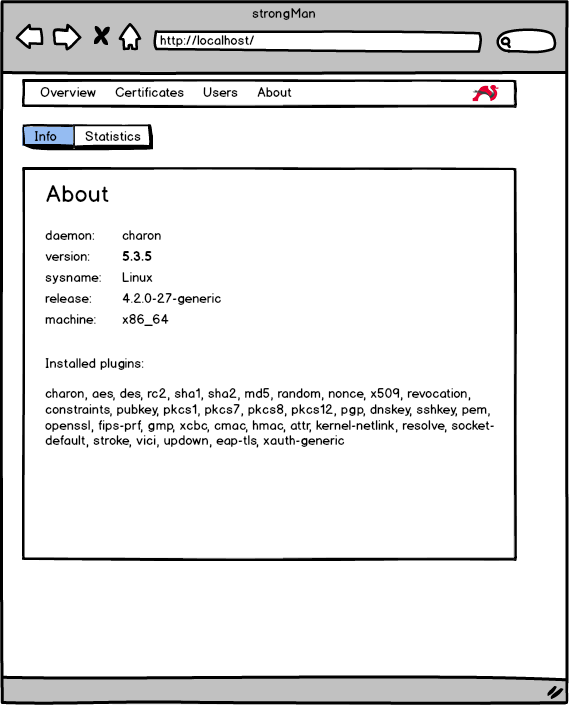
\includegraphics[width=400pt]{images/mockups/About.png}
	\caption{About}
\end{figure}

\begin{figure}[H]
	\centering
	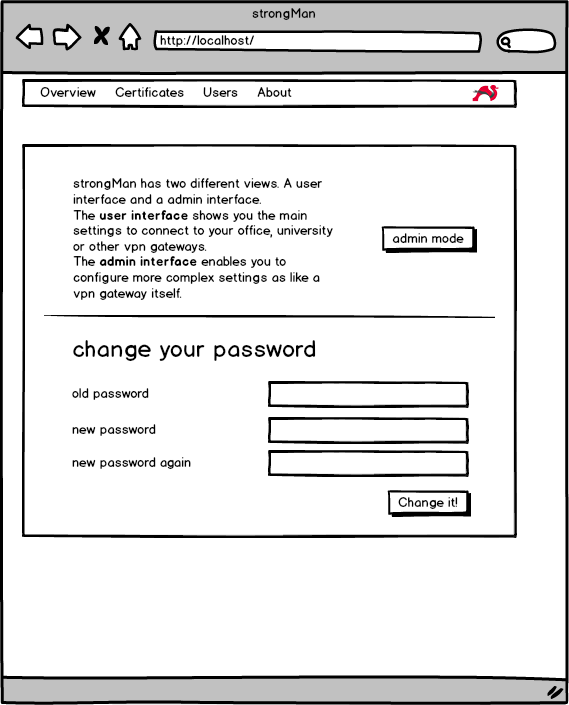
\includegraphics[width=400pt]{images/mockups/user_pw_change.png}
	\caption{User page}
\end{figure}

\newpage
\chapter{Inhalt der CD}
Der Inhalt der CD glieder sich folgendermassen:
\begin{figure}[H]
\dirtree{%
.1 CD.
.2 Studienarbeit.pdf.
.2 0\_AUFGABE.
.3 Original Aufgabenstellung.
.2 1\_CODE.
.3 GitHub Repository.
.2 2\_DOKUMENTATION.
.3 Protokolle.
.3 Poster.
}
\end{figure}
\newpage

\chapter{Eigenständigkeitserklärung}

Wir erklären hiermit,
\begin{itemize}
	\item dass wir die vorliegende Arbeit selber und ohne fremde Hilfe durchgeführt haben, ausser derjenigen, welche explizit in der Aufgabenstellung erwähnt sind oder mit dem Betreuer schriftlich vereinbart wurden.
	\item dass wir sämtliche verwendeten Quellen erwähnt und gemäss gängigen wissenschaftlichen Zitierregeln korrekt angegeben haben.
	\item dass wir keine durch Copyright geschützten Materialien (z.B. Bilder) in dieser Arbeit in unerlaubter Weise genutzt haben.
\end{itemize}

\vspace{2cm}

Ort, Datum:

\begin{itemize}
	\item[] Rapperswil, \today
\end{itemize}


\vspace{1cm}
Namen, Unterschriften:
\vspace{2cm}
\begin{tabbing}[H]
    \hspace*{1cm}\=\hspace*{8cm}\=\hspace*{6cm}\= \kill
     \> Severin Bühler \> Samuel Kurath \\
\end{tabbing}

\begingroup     
\let\clearpage\relax        
\printglossary[title=\chapter{Glossar}]
\endgroup
% Bibliography
%%%%%%%%%%%%%%
\bibliographystyle {alpha}
\bibliography{index/bibliography}



% List of figures, tables and descision
\listoffigures
\newpage
\listoftables
\newpage
\listofdecision
\newpage

\end{document}

